\documentclass[UTF8]{ctexart}
\usepackage{geometry}
\usepackage{titlesec}
\usepackage{graphicx}
\usepackage{fancyhdr}
\usepackage{ragged2e}
\usepackage{anyfontsize}
\usepackage{tikz}
\usepackage{float}
\usetikzlibrary{shapes,arrows,positioning,calc}
\usepackage{array}
\usepackage{enumerate}
\usepackage{listings}
\usepackage{color}
\usepackage{lineno}
\usepackage[hidelinks]{hyperref}
\makeatletter
\newlength\underlineMinSep
\setlength\underlineMinSep{1em}
\newcommand\underlineX[1]{%
  \hskip\underlineMinSep
  \begin{minipage}[t]{10cm}
    \centering
    % see `texdoc lineno`, sec. 7.4
    \internallinenumbers
    \renewcommand\makeLineNumber{\hss
      \rlap{\hskip-\underlineMinSep
        \rule[.5\dimexpr\f@size pt-\baselineskip]{\dimexpr\textwidth+2\underlineMinSep}{.4pt}}}%
    #1
  \end{minipage}%
}
\makeatother
\geometry{a4paper, left=30mm, right=30mm, top=40mm, bottom=40mm,headheight=16pt}



\renewcommand{\maketitle}[5]{
\begin{titlepage}
    \LARGE\centering{\textbf{南\hspace{1em}京\hspace{1em}师\hspace{1em}范\hspace{1em}大\hspace{1em}学}}
    \\
    \vspace{1cm}
    \Huge\centering{\textbf{#1}}
    \vspace{1cm}
    \begin{center}
        \includegraphics{../njnu.jpg}
    \end{center}
    \vspace{1cm}
    \begin{tabular}{@{}c@{}c@{}}
        \Large\textbf{题\hspace{2em}目:} & \Large\underlineX{#2} \\
        \Large\textbf{学\hspace{2em}院:} & \Large\underlineX{计算机与电子信息/人工智能学院}\\
        \Large\textbf{专\hspace{2em}业:} & \Large\underlineX{计算机科学与技术} \\
        \Large\textbf{小组成员:} & \Large\underlineX{#3} \\
        \Large\textbf{指导教师:} & \Large\underlineX{#4} \\
    \end{tabular}\\
    \vspace{1cm}
    \centering{\textbf{\large{#5}}}
    \newpage
\end{titlepage}
}

\newcommand{\subsubsubsection}[1]{\paragraph{#1}\mbox{}\\} % 把paragraph命令重命名为\subsubsubsection
\setcounter{secnumdepth}{4} % 添加标号
\setcounter{tocdepth}{4} % 添加到目录中

\newcommand{\subsubsubsubsection}[1]{\subparagraph{#1}\mbox{}\\} % 把subparagraph命令重命名为\subsubsubsubsection
\setcounter{secnumdepth}{5} % 添加标号
\setcounter{tocdepth}{5} % 添加到目录中



% 设置页眉页脚
\pagestyle{fancy}
\fancyhf{}
\fancyhead[R]{\bfseries\leftmark}
\fancyfoot[C]{\bfseries\thepage}
\renewcommand{\headrulewidth}{0.5pt} 
\renewcommand{\footrulewidth}{0pt}
    

\begin{document}
\maketitle{《软件工程》课程设计}{企业级BBS系统}{张桂楠\hspace{0.5em}余睿\hspace{0.5em}纪安东\hspace{0.5em}李绍东\hspace{0.5em}王双阳\hspace{0.5em}顾逸}{杨俊}{2024年5月15日}


\tableofcontents

\newpage
\section{系统目标}

企业级BBS系统是一个面向企业内部员工的论坛系统,用于员工之间的交流和沟通。系统的目标是提供一个安全、高效、易用的论坛系统,以促进企业内部员工之间的交流和沟通。系统的主要功能包括用户账户管理、帖子管理、评论管理、板块管理等。系统的主要用户是企业内部员工,他们可以通过系统发布帖子、评论帖子、查看帖子等。系统的主要功能包括用户账户管理、帖子管理、评论管理、板块管理等。系统的主要用户是企业内部员工,他们可以通过系统发布帖子、评论帖子、查看帖子等。


\newpage
\section{需求分析}

\subsection{功能分析}

\subsubsection{功能描述}

\subsubsubsection{用户功能}

1. 功能描述
\begin{itemize}
  \item 用户注册:用户可以通过注册功能创建一个新的账户。
  \item 用户登录:用户可以通过登录功能登录到系统。
\end{itemize}

2. 用户账户管理用例图
\begin{figure}[H]
  \centering
  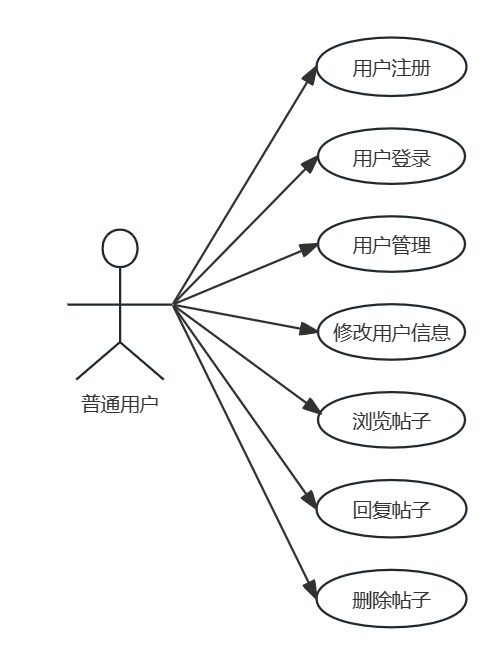
\includegraphics[scale=0.3]{用例图/普通用户用例图.jpg}
  \caption{用户账户管理用例图}
\end{figure}

3. 用户账户管理活动图
\begin{figure}[H]
  \centering
  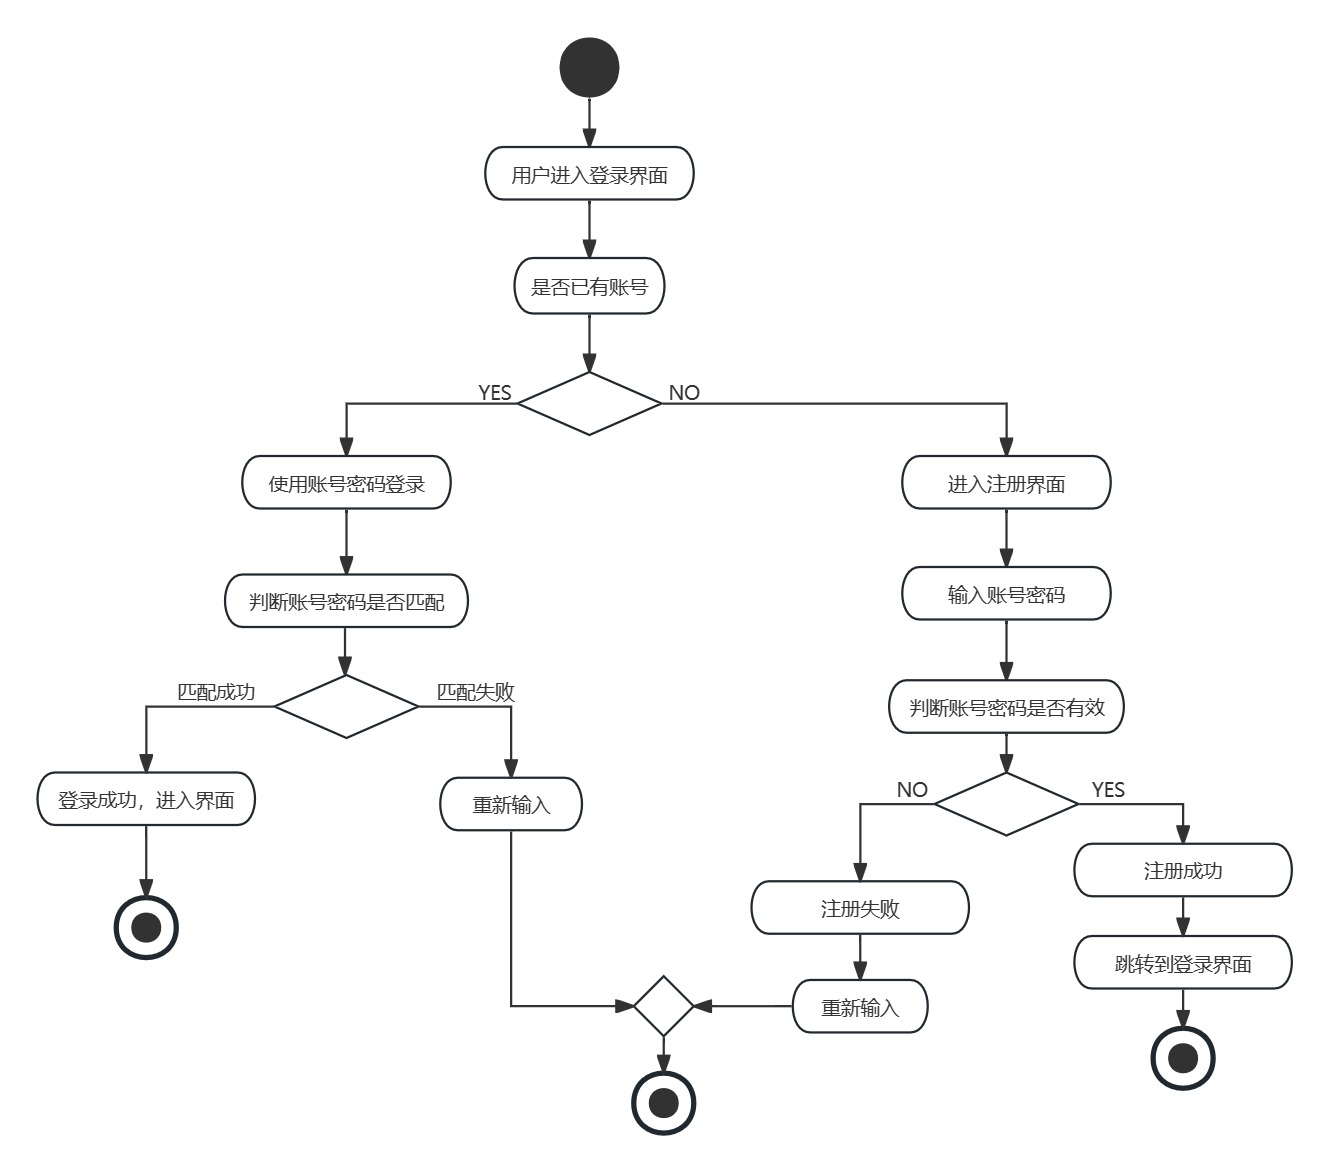
\includegraphics[scale=0.25]{活动图/用户账户管理活动图.jpg}
  \caption{用户账户管理活动图}
\end{figure}

\begin{figure}[H]
  \centering
  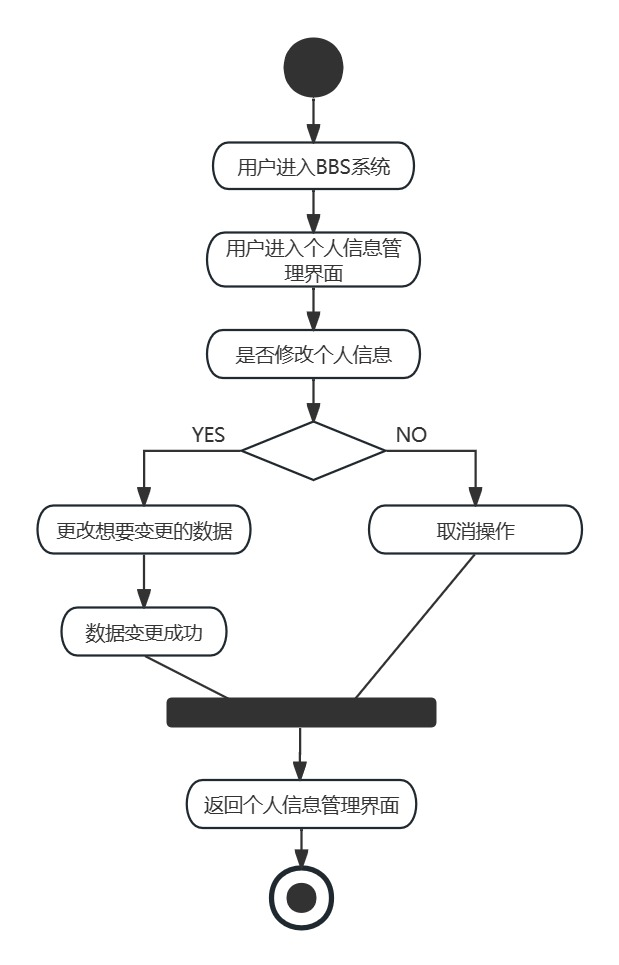
\includegraphics[scale=0.25]{活动图/用户修改个人信息活动图.jpg}
  \caption{用户修改个人信息活动图}
\end{figure}

\begin{figure}[H]
  \centering
  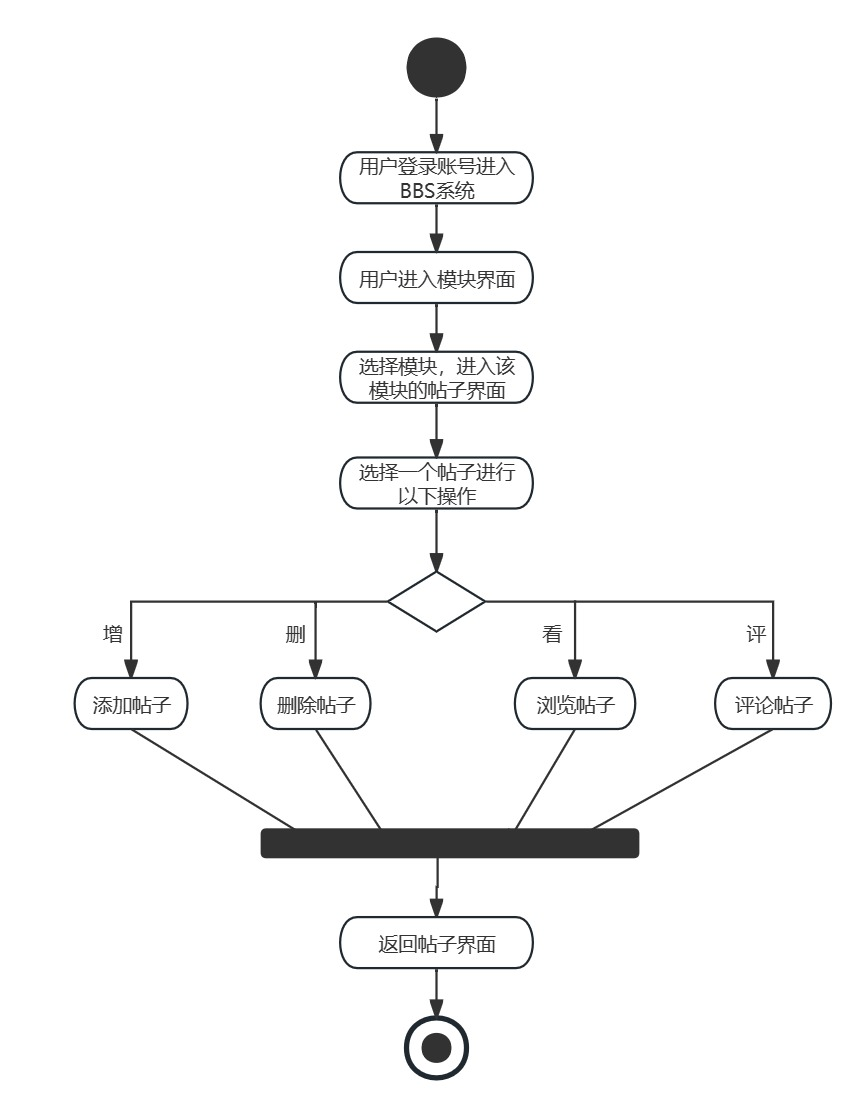
\includegraphics[scale=0.25]{活动图/用户帖子操作活动图.jpg}
  \caption{用户帖子操作活动图}
\end{figure}

\begin{figure}[H]
  \centering
  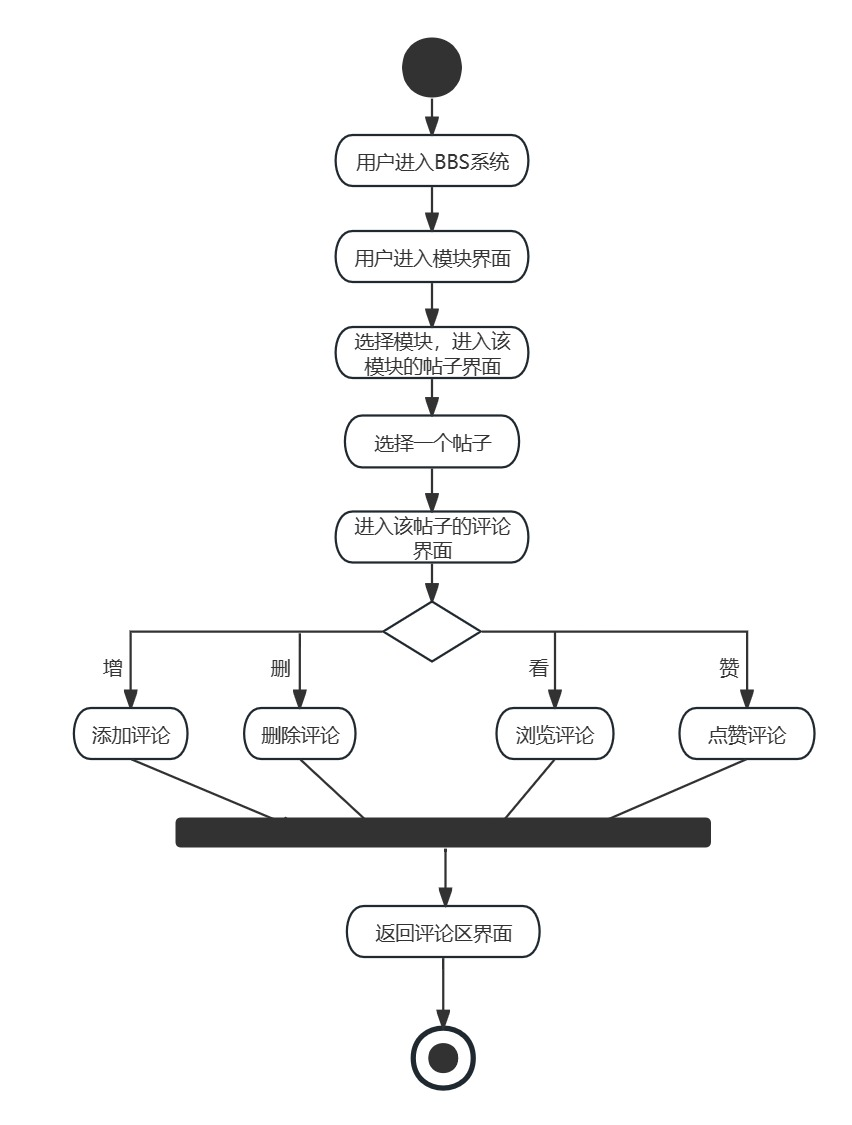
\includegraphics[scale=0.25]{活动图/用户评论操作活动图.jpg}
  \caption{用户评论操作活动图}
\end{figure}

\subsubsubsection{管理员功能}

1. 功能描述
\begin{itemize}
  \item 管理员登录:管理员可以通过登录功能登录到系统。
\end{itemize}

2. 管理员账户管理用例图
\begin{figure}[H]
  \centering
  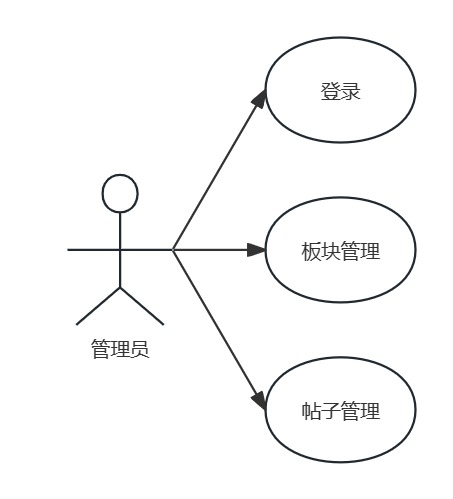
\includegraphics[scale=0.3]{用例图/管理员用例图.jpg}
  \caption{管理员账户管理用例图}
\end{figure}

3. 管理员账户管理活动图
\begin{figure}[H]
  \centering
  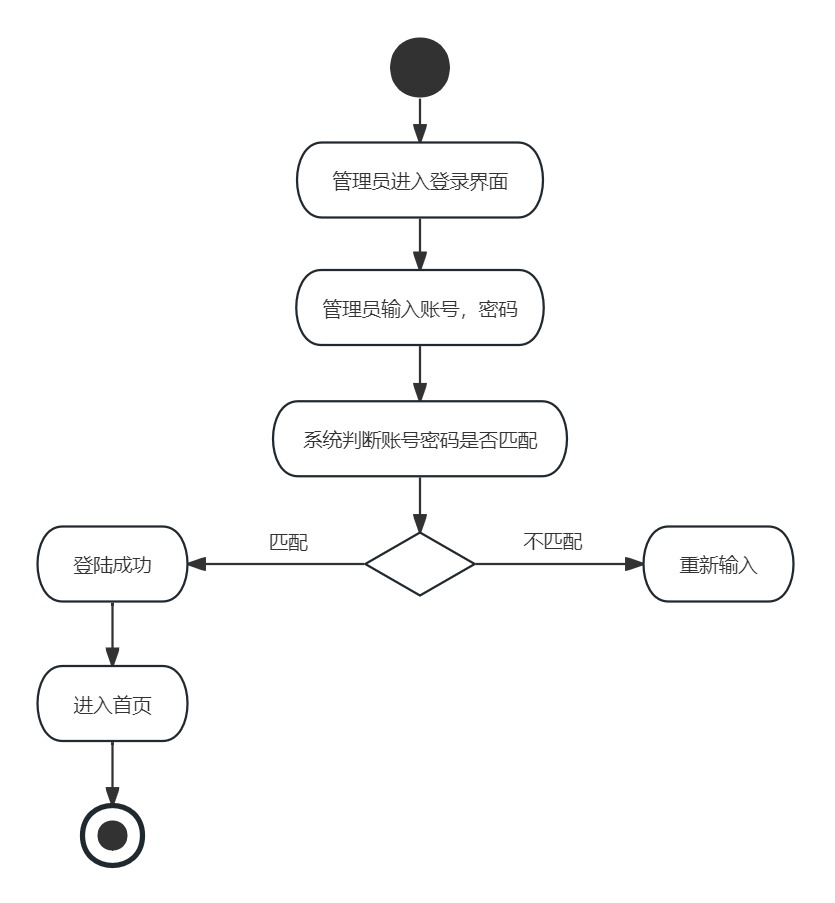
\includegraphics[scale=0.25]{活动图/管理员登录活动图.jpg}
  \caption{用户登录活动图}
\end{figure}

\begin{figure}[H]
  \centering
  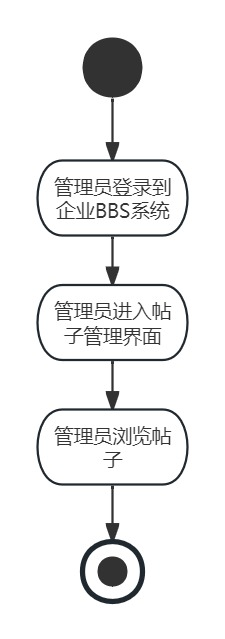
\includegraphics[scale=0.25]{活动图/管理员浏览帖子活动图.jpg}
  \caption{管理员浏览帖子活动图}
\end{figure}

\begin{figure}[H]
  \centering
  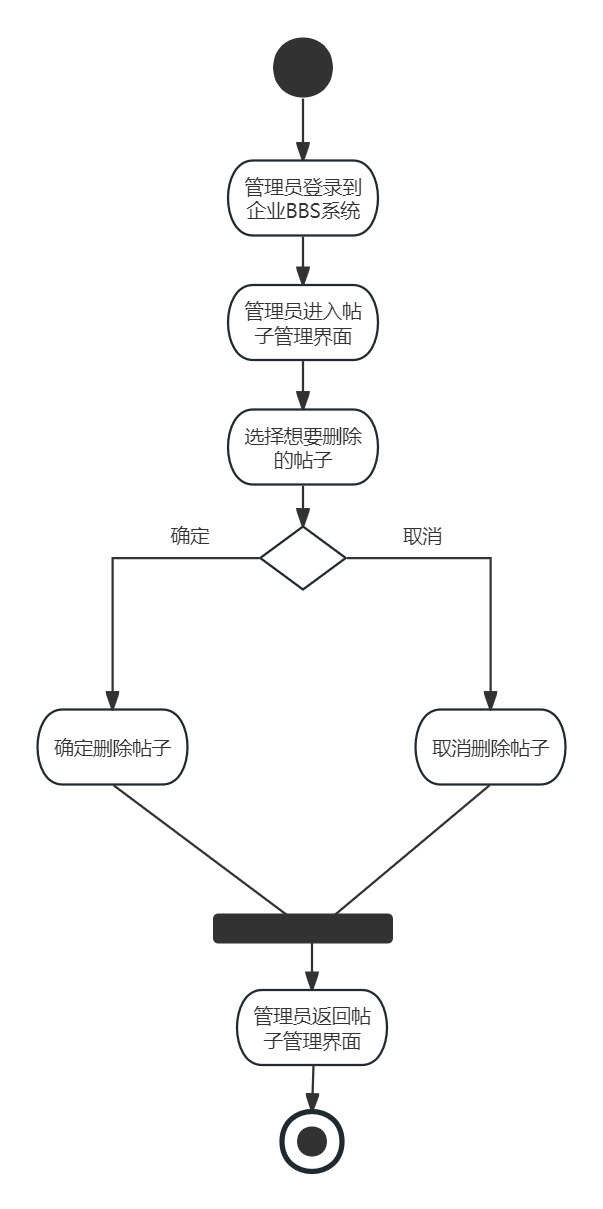
\includegraphics[scale=0.25]{活动图/管理员删除帖子活动图.jpg}
  \caption{管理员删除帖子活动图}
\end{figure}

\begin{figure}[H]
  \centering
  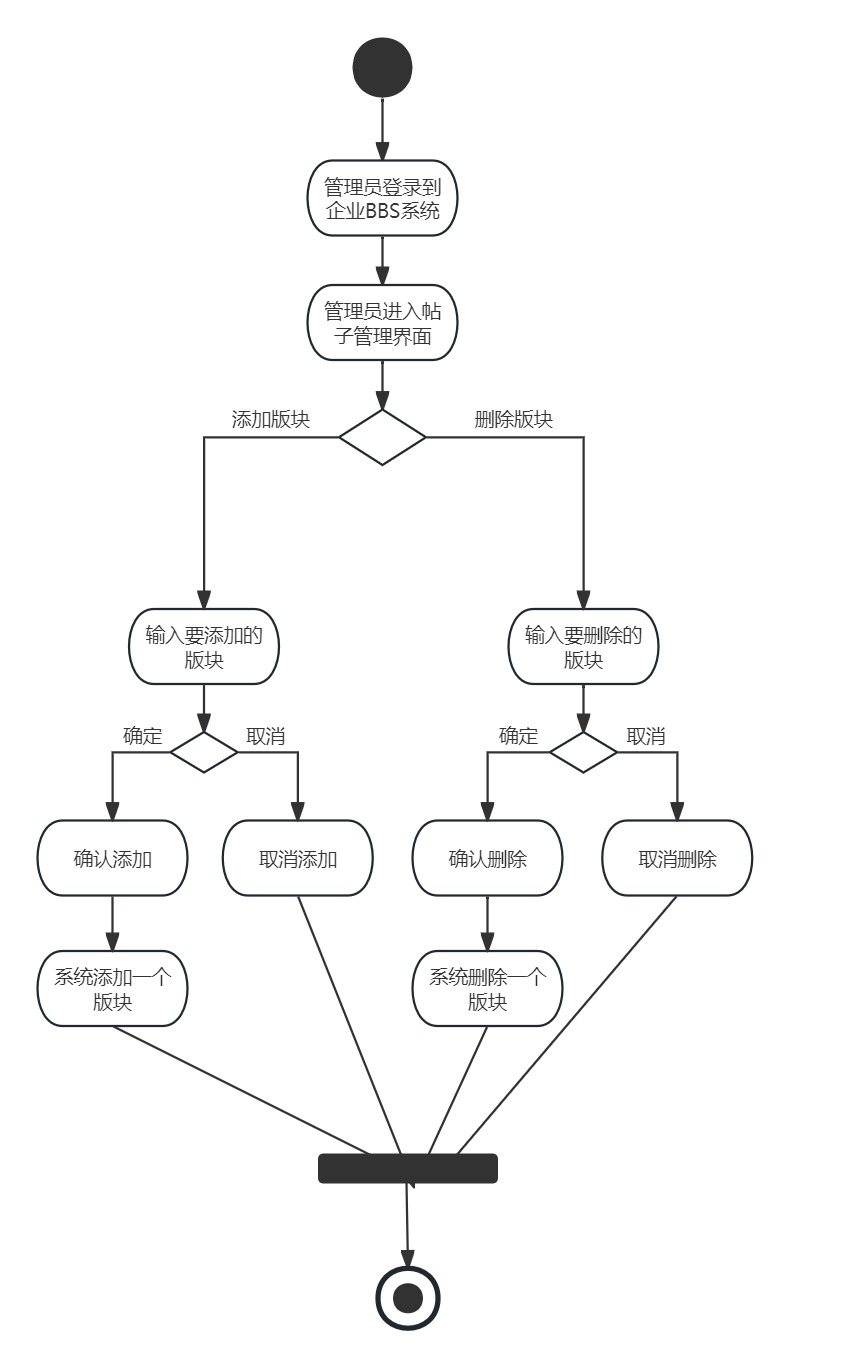
\includegraphics[scale=0.25]{活动图/管理员版块管理活动图.jpg}
  \caption{管理员版块管理活动图}
\end{figure}




\newpage

\subsubsection{逻辑分析与建模}

\subsubsubsection{用户账户管理}

1.类分析
\begin{itemize}
  \item 边界类:登录界面类、注册界面类
  \item 控制类:登录控制类、注册控制类
  \item 实体类:用户列表类、用户类
\end{itemize}

2.类模型图

\begin{figure}[H]
  \centering
  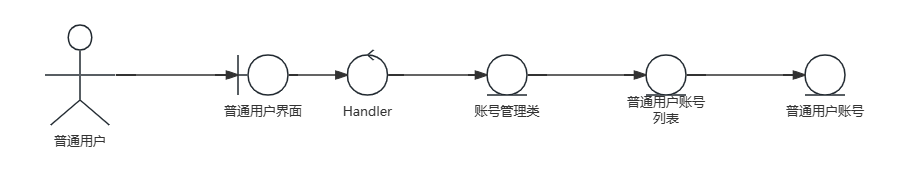
\includegraphics[scale=0.3]{类图/用户账号.png}
  \caption{用户账户管理类模型图}
\end{figure}
3.协作图

\begin{figure}[H]
  \centering
  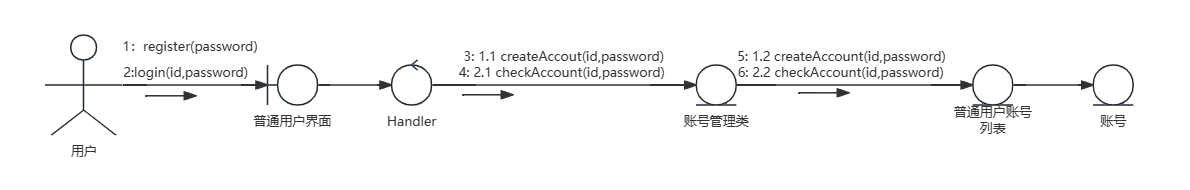
\includegraphics[scale=0.3]{协作图/用户账号.png}
  \caption{用户账户管理协作图}
\end{figure}



\subsubsubsection{帖子管理}

1.类分析
\begin{itemize}
  \item 边界类:帖子管理界面类
  \item 控制类:帖子管理控制类
  \item 实体类:帖子类、帖子列表类
\end{itemize}

2.类模型图

\begin{figure}[H]
  \centering
  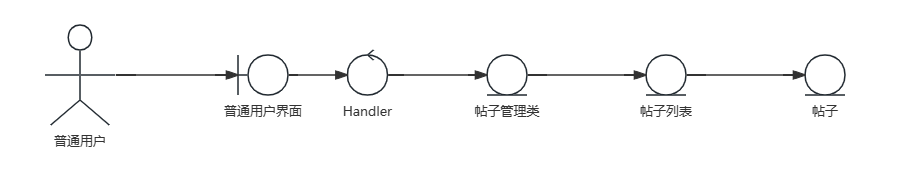
\includegraphics[scale=0.3]{类图/用户帖子管理.png}
  \caption{帖子管理类模型图}
\end{figure}


3.协作图

\begin{figure}[H]
  \centering
  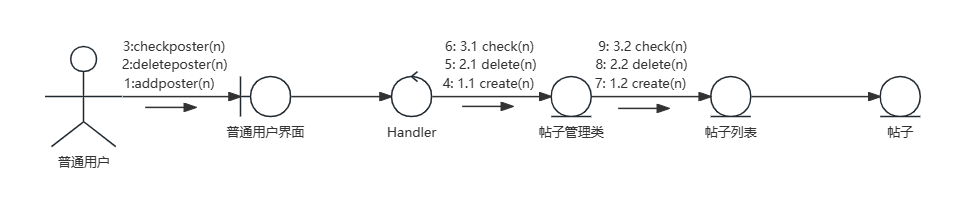
\includegraphics[scale=0.3]{协作图/用户帖子.png}
  \caption{帖子管理协作图}
\end{figure}




\subsubsubsection{帖子回复管理}

1.类分析
\begin{itemize}
  \item 边界类:帖子回复管理界面类
  \item 控制类:帖子回复管理控制类
  \item 实体类:回复类、回复列表类
\end{itemize}

2.类模型图

\begin{figure}[H]
  \centering
  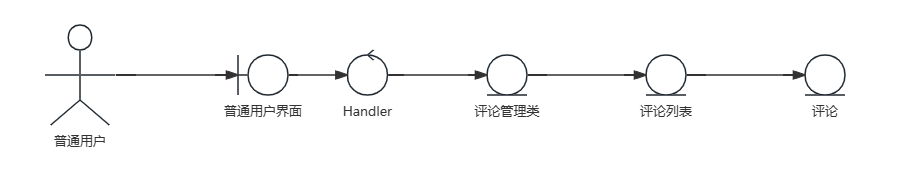
\includegraphics[scale=0.3]{类图/用户评论.png}
  \caption{帖子回复管理类模型图}
\end{figure}


3.协作图

\begin{figure}[H]
  \centering
  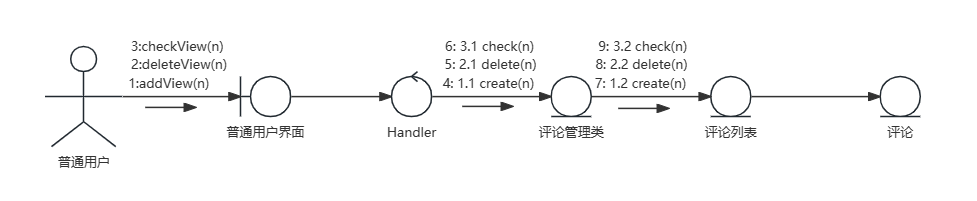
\includegraphics[scale=0.3]{协作图/用户评论.png}
  \caption{帖子回复管理协作图}
\end{figure}


\subsubsubsection{管理员账户管理}

1.类分析
\begin{itemize}
  \item 边界类:登录界面类
  \item 控制类:登录控制类
  \item 实体类:管理员列表类、管理员类
\end{itemize}

2.类模型图

\begin{figure}[H]
  \centering
  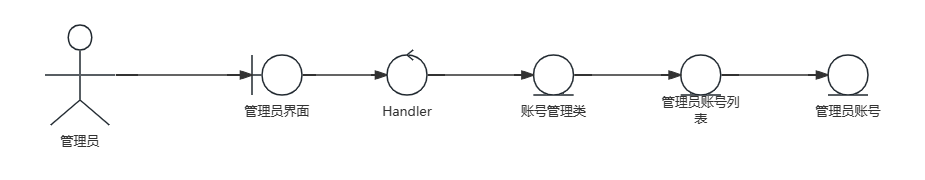
\includegraphics[scale=0.3]{类图/管理员账号.png}
  \caption{管理员账户管理类模型图}
\end{figure}
3.协作图

\begin{figure}[H]
  \centering
  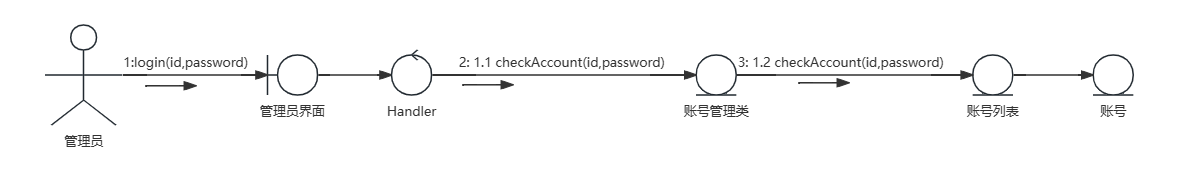
\includegraphics[scale=0.3]{协作图/管理员账号.png}
  \caption{管理员账户管理协作图}
\end{figure}


\subsubsubsection{管理员帖子模块管理}

1.类分析
\begin{itemize}
  \item 边界类:管理员帖子模块管理界面类
  \item 控制类:管理员帖子模块管理控制类
  \item 实体类:帖子模块列表类、帖子模块类
\end{itemize}

2.类模型图

\begin{figure}[H]
  \centering
  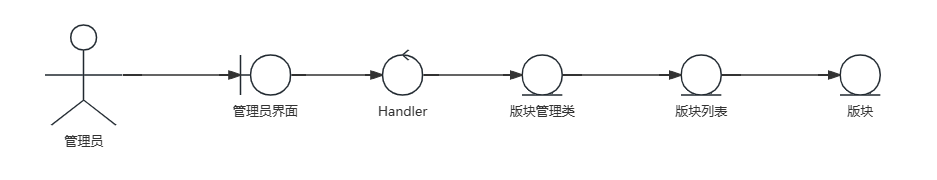
\includegraphics[scale=0.3]{类图/管理员版块管理.png}
  \caption{管理员帖子模块管理类模型图}
\end{figure}

3.协作图

\begin{figure}[H]
  \centering
  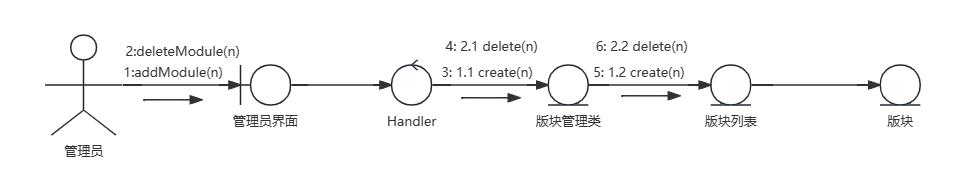
\includegraphics[scale=0.3]{协作图/管理版块.png}
  \caption{管理员帖子模块管理协作图}
\end{figure}

\subsubsubsection{管理员帖子管理}

1.类分析
\begin{itemize}
  \item 边界类:管理员帖子管理界面类
  \item 控制类:管理员帖子管理控制类
  \item 实体类:帖子列表类、帖子类
\end{itemize}

2.类模型图

\begin{figure}[H]
  \centering
  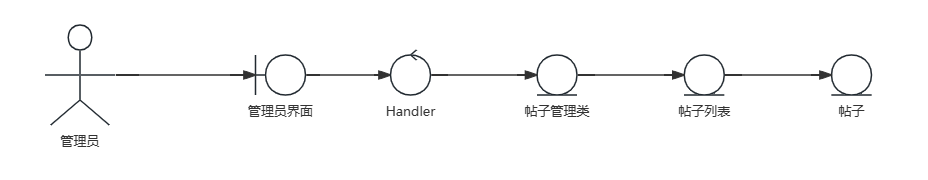
\includegraphics[scale=0.3]{类图/管理员帖子管理.png}
  \caption{管理员帖子管理类模型图}
\end{figure}

3.协作图

\begin{figure}[H]
  \centering
  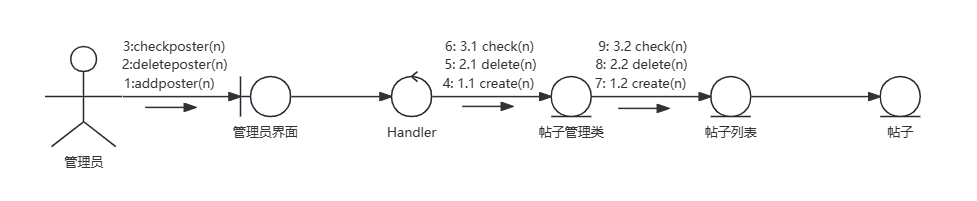
\includegraphics[scale=0.3]{协作图/管理员帖子.png}
  \caption{管理员帖子管理协作图}
\end{figure}



\newpage
\subsection{非功能分析}

\subsubsection{性能需求}
\begin{enumerate}
  \item 系统应该具有良好的性能,以便用户可以发布帖子、评论帖子、查看帖子等。
\end{enumerate}

\subsubsection{安全性需求}
\begin{enumerate}
  \item 用户数据应该得到保护,确保用户数据不会被泄露。
\end{enumerate}

\subsubsection{可靠性需求}
\begin{enumerate}
  \item 系统应该可靠,最小化系统宕机或故障的时间。
\end{enumerate}

\subsubsection{可用性需求}
\begin{enumerate}
 \item 系统应该具有良好的可用性,以便用户可以轻松地使用系统。
\end{enumerate}

\subsubsection{可维护性需求}
\begin{enumerate}
  \item 系统应该具有良好的可维护性,以便在需要时能够轻松地对其进行修改和维护。
\end{enumerate}

\subsubsection{可拓展性需求}
\begin{enumerate}
  \item 系统应该支持扩展以增加新功能和模块。 
\end{enumerate}

\newpage
\section{系统设计}
\subsection{功能划分}
\subsubsection{用户账户管理}
\begin{itemize}
  \item 用户注册:用户可以通过注册页面,输入注册账号密码,注册账号
  \item 用户登录:用户可以通过登录页面,输入账号密码,登录账号
\end{itemize}

\subsubsection{帖子管理}
\begin{itemize}
  \item 帖子发布:用户可以发布新的帖子
  \item 帖子浏览:用户可以浏览帖子
  \item 帖子编辑:用户可以编辑帖子的内容
  \item 帖子删除:用户可以删除帖子
\end{itemize}

\subsubsection{帖子回复管理}
\begin{itemize}
  \item 回复帖子:用户可以回复帖子
  \item 删除回复:用户可以删除回复
  \item 编辑回复:用户可以编辑回复
  \item 查看回复:用户可以查看回复
\end{itemize}

  
\subsubsection{帖子模块管理}
\begin{itemize}
  \item 管理员可以对帖子模块进行管理,包括查看帖子模块、添加帖子模块、删除帖子模块、编辑帖子模块
\end{itemize}


\subsection{功能设计}

\subsubsection{账户管理}

\subsubsubsection{用户注册和登录精细类图}

\begin{figure}[H]
  \centering
  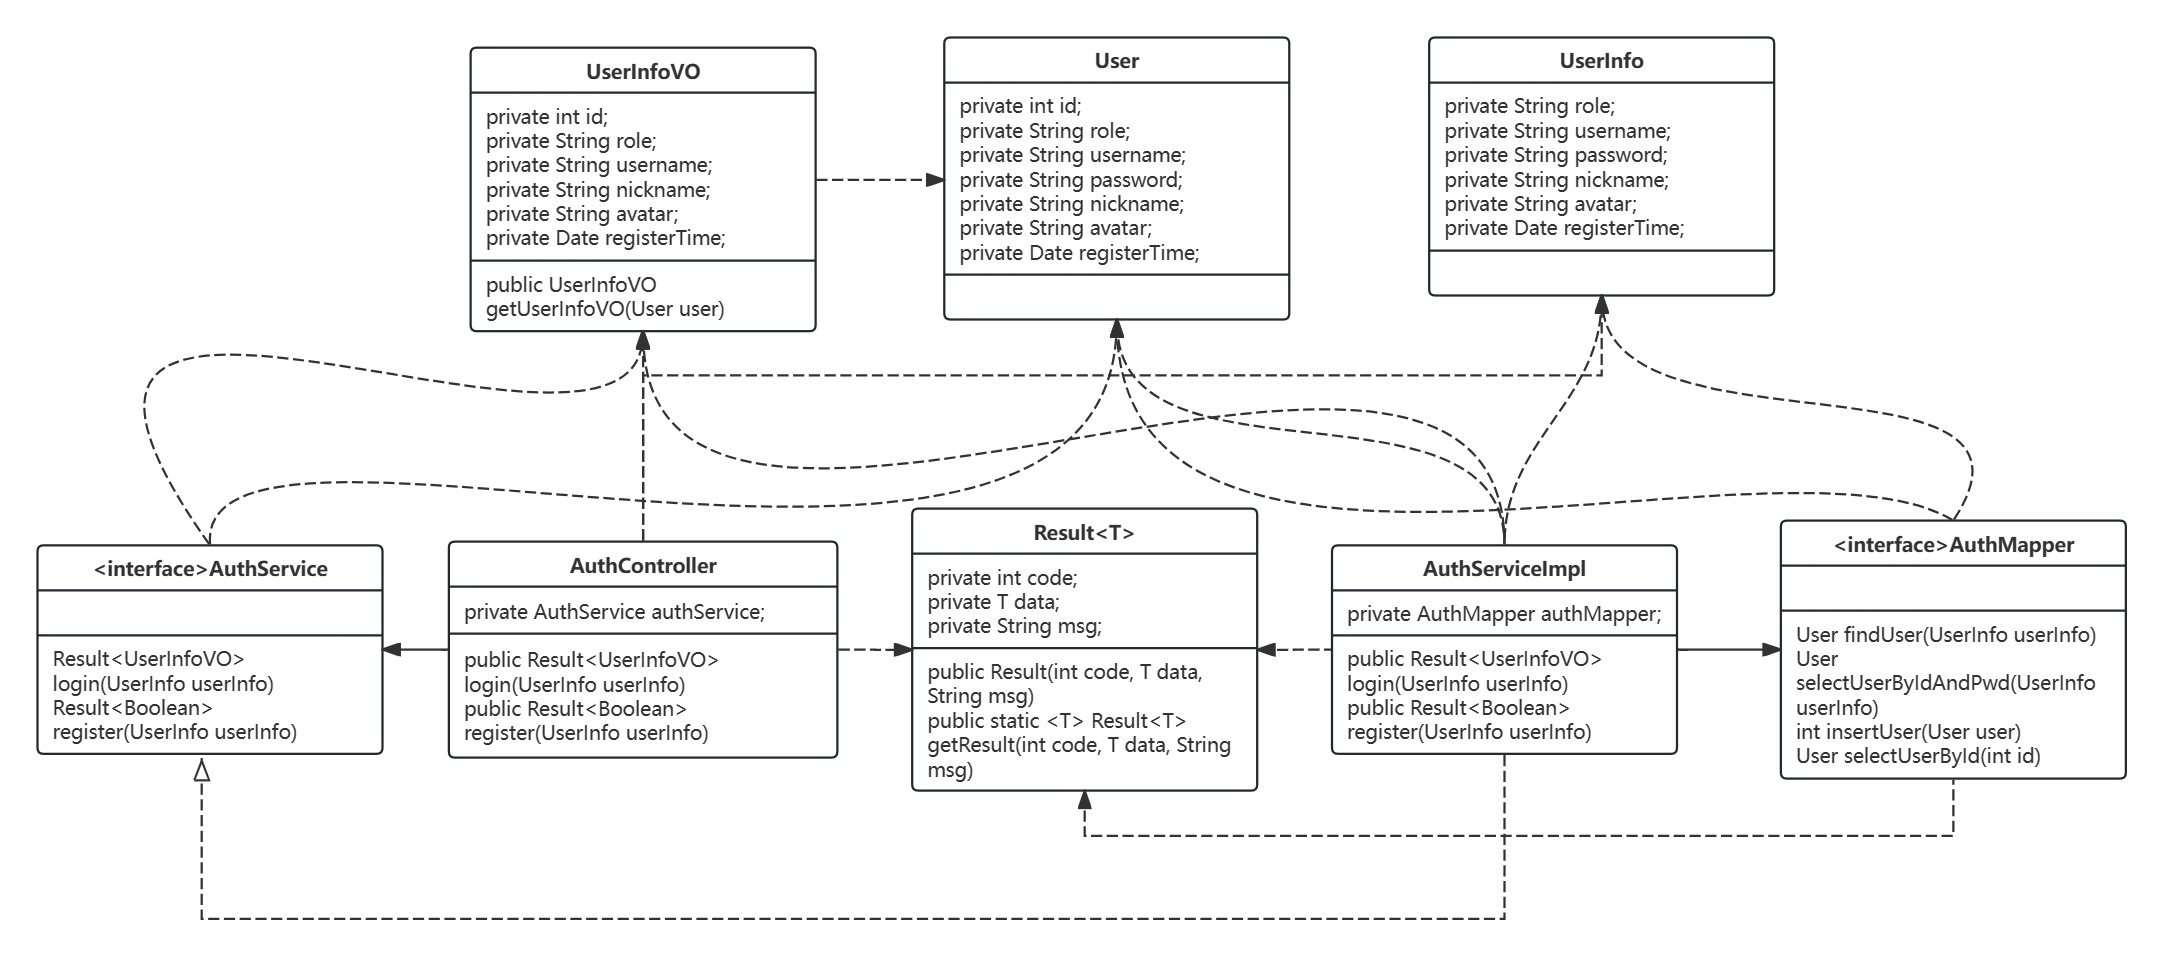
\includegraphics[scale=0.2]{精化类模型图/auth.jpg}
  \caption{用户注册和登录类图}
\end{figure}


\subsubsubsection{注册和登录时序图}

\begin{figure}[H]
  \centering
  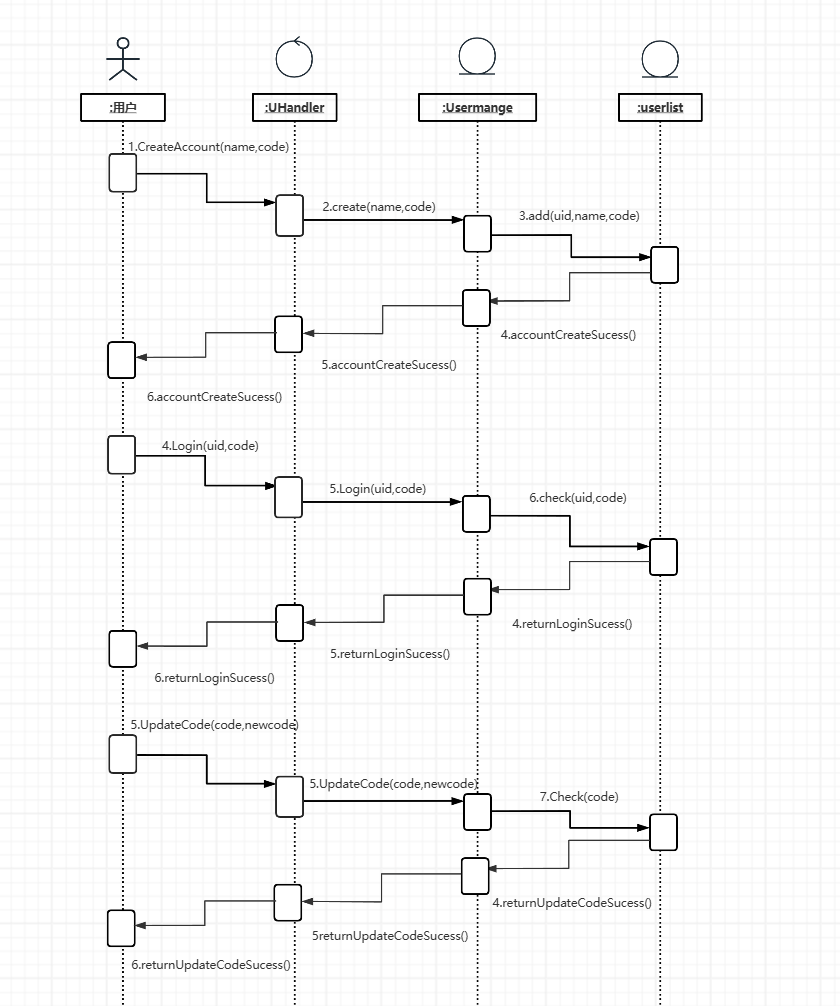
\includegraphics[scale=0.3]{顺序图/用户登录注册.png}
  \caption{用户注册时序图}
\end{figure}

\begin{figure}[H]
  \centering
  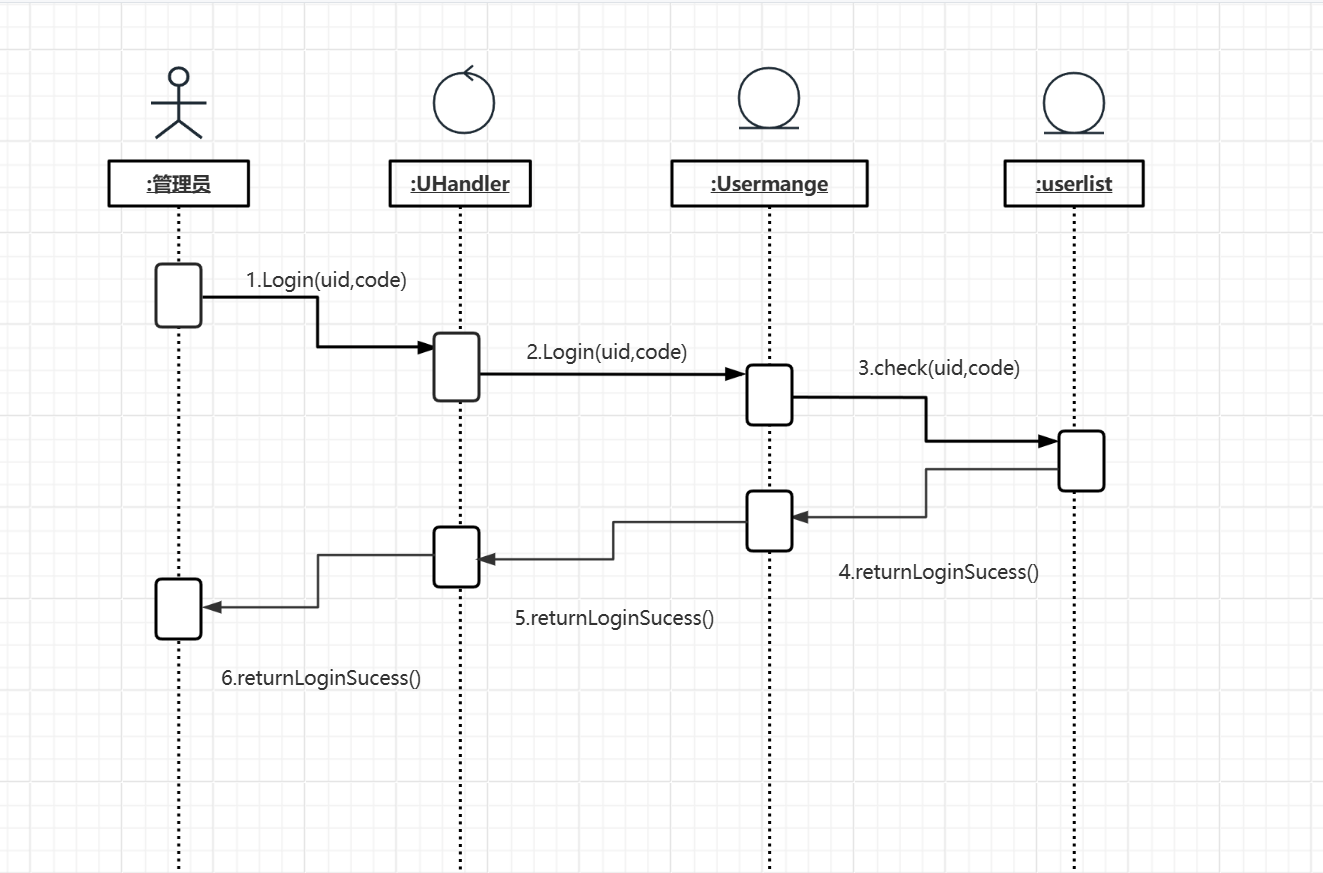
\includegraphics[scale=0.3]{顺序图/管理员登录.png}
  \caption{管理员登录时序图}
\end{figure}


\subsubsection{帖子管理}

\subsubsubsection{帖子发布和浏览精细类图}

\begin{figure}[H]
  \centering
  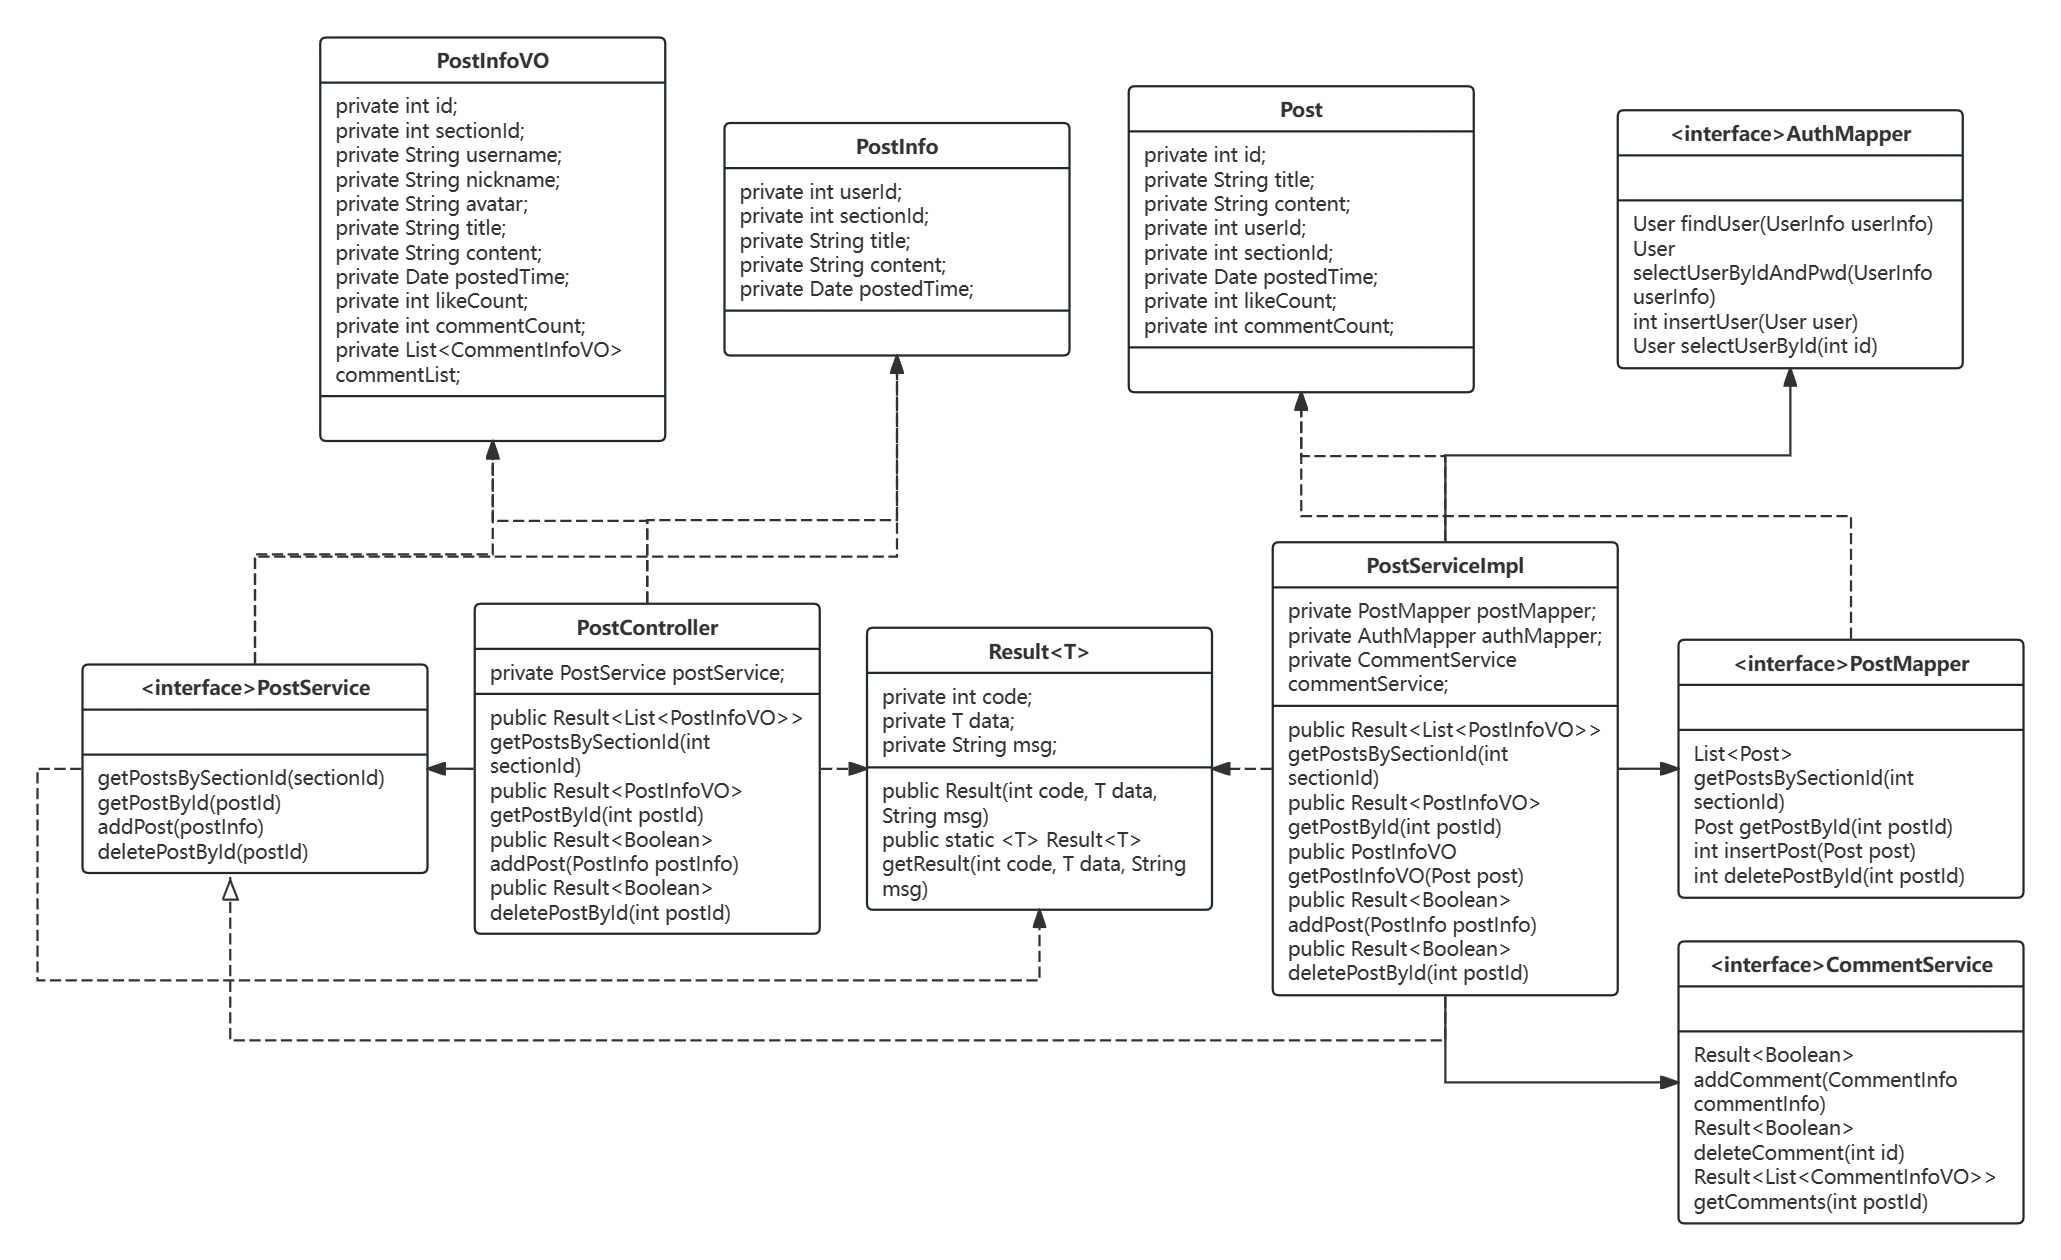
\includegraphics[scale=0.2]{精化类模型图/Post.jpg}
  \caption{帖子发布和浏览类图}
\end{figure}

\subsubsubsection{帖子发布和浏览时序图}

\begin{figure}[H]
  \centering
  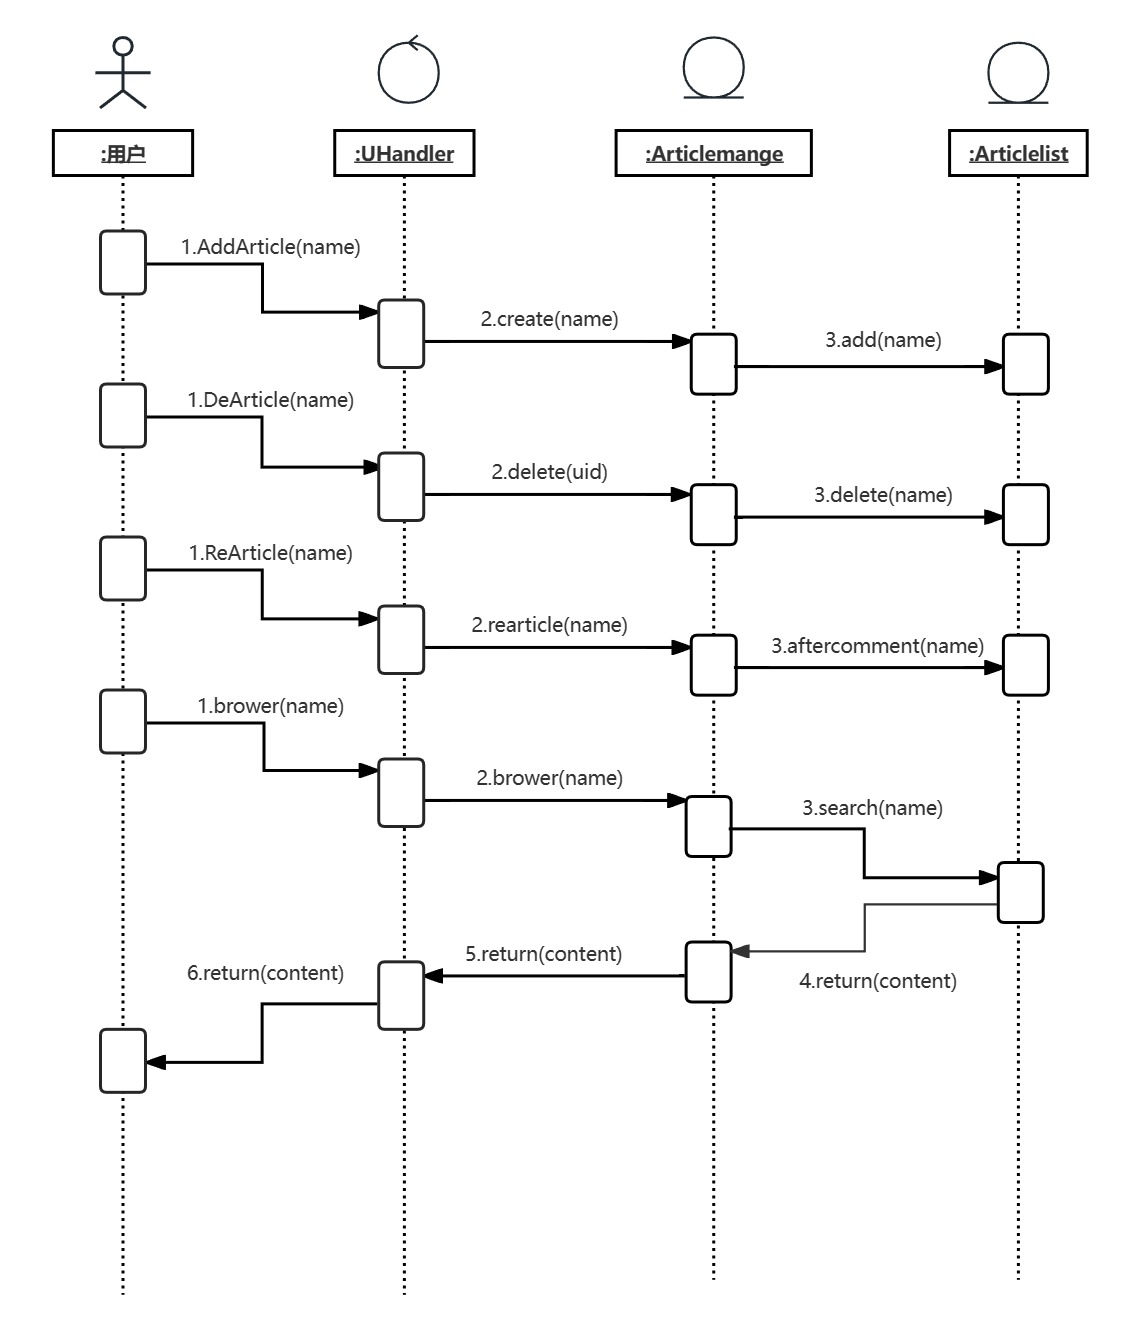
\includegraphics[scale=0.3]{顺序图/普通用户发帖.png}
  \caption{普通用户发帖时序图}
\end{figure}


\begin{figure}[H]
  \centering
  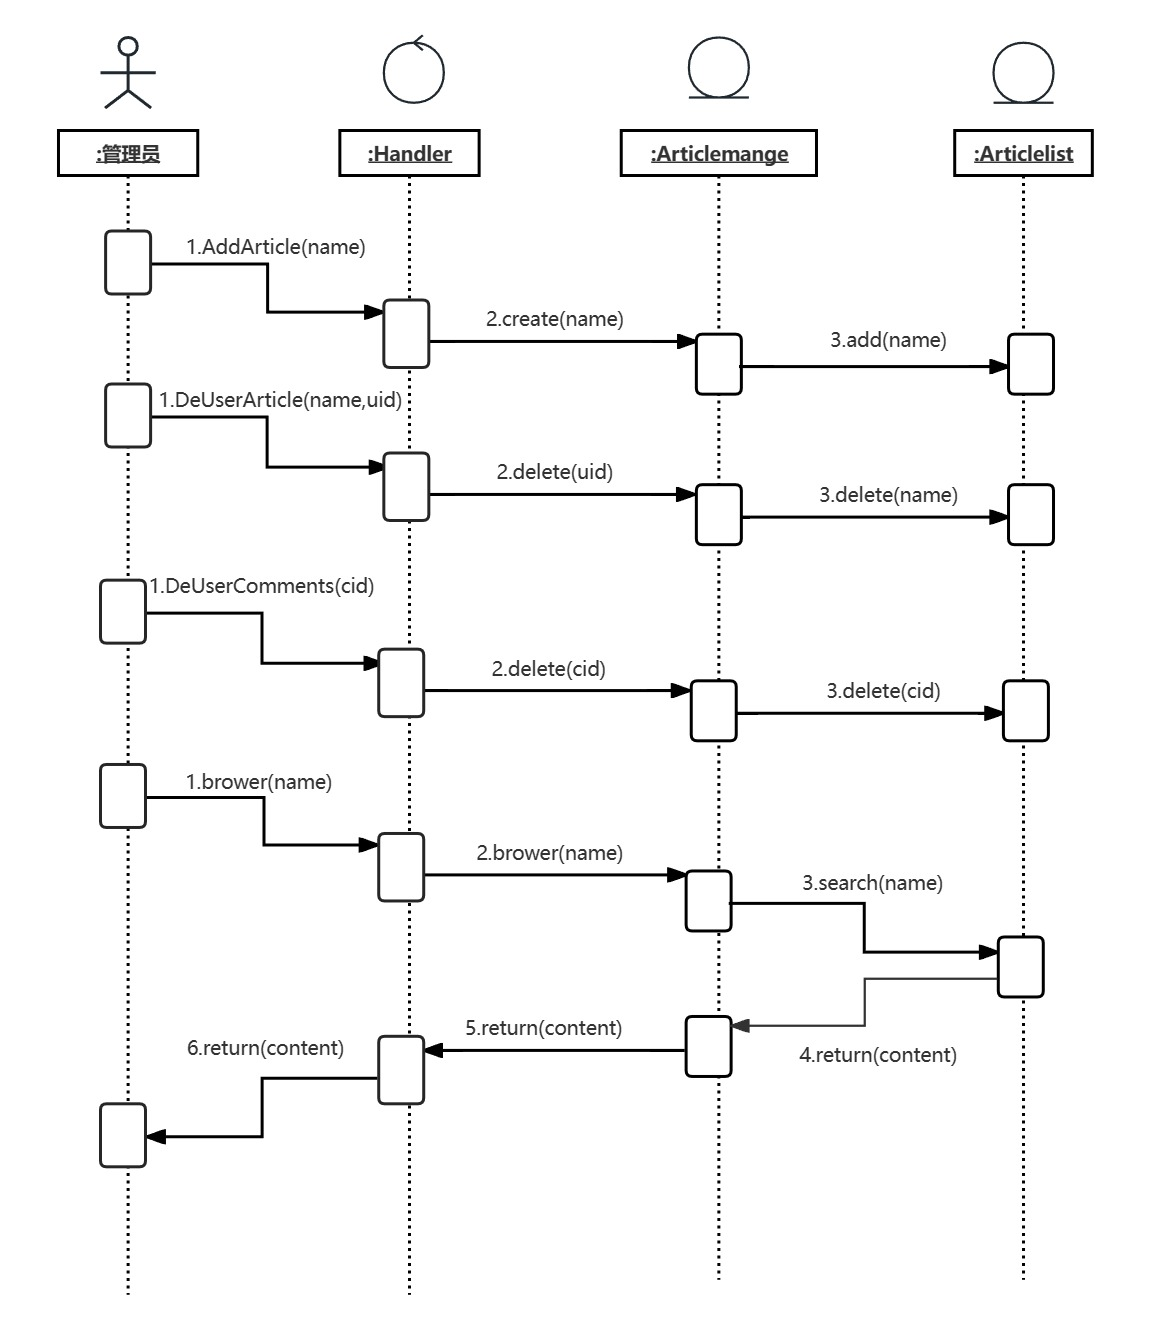
\includegraphics[scale=0.3]{顺序图/管理员发帖.png}
  \caption{管理员发帖}
\end{figure}



\subsubsection{评论管理}

\subsubsubsection{评论发布和浏览精细类图}

\begin{figure}[H]
  \centering
  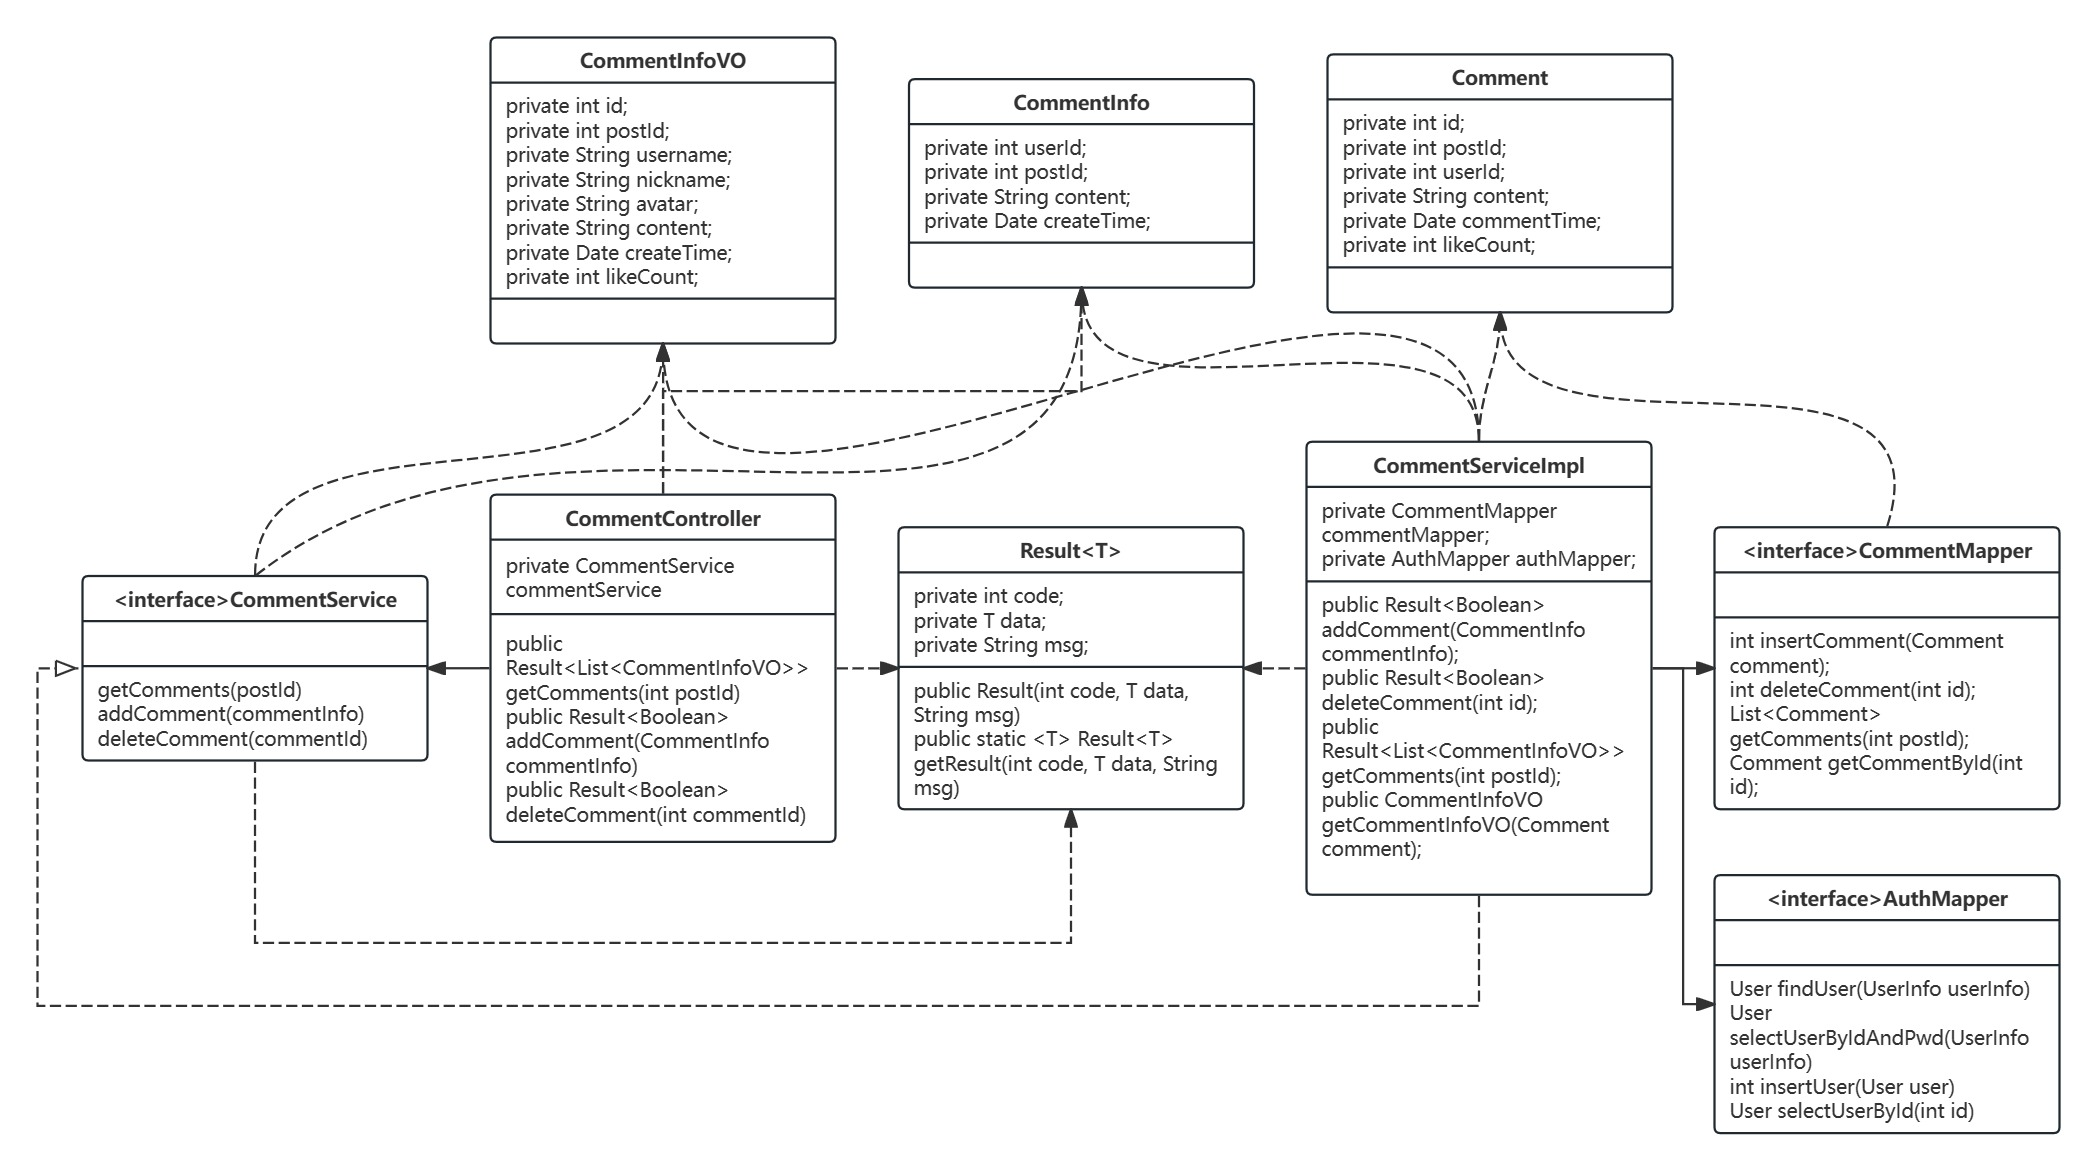
\includegraphics[scale=0.2]{精化类模型图/comment.jpg}
  \caption{评论发布和浏览类图}
\end{figure}

\subsubsubsection{评论发布和浏览时序图}

\begin{figure}[H]
  \centering
  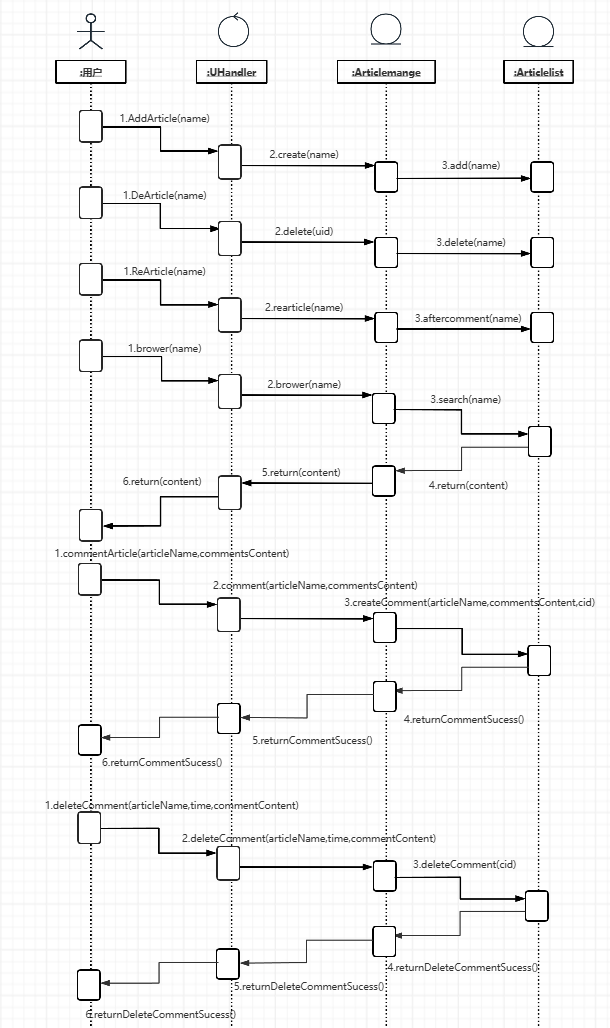
\includegraphics[scale=0.3]{顺序图/用户评论.png}
  \caption{用户评论时序图}
\end{figure}



\subsubsection{模块管理}

\subsubsubsection{模块管理精细类图}

\begin{figure}[H]
  \centering
  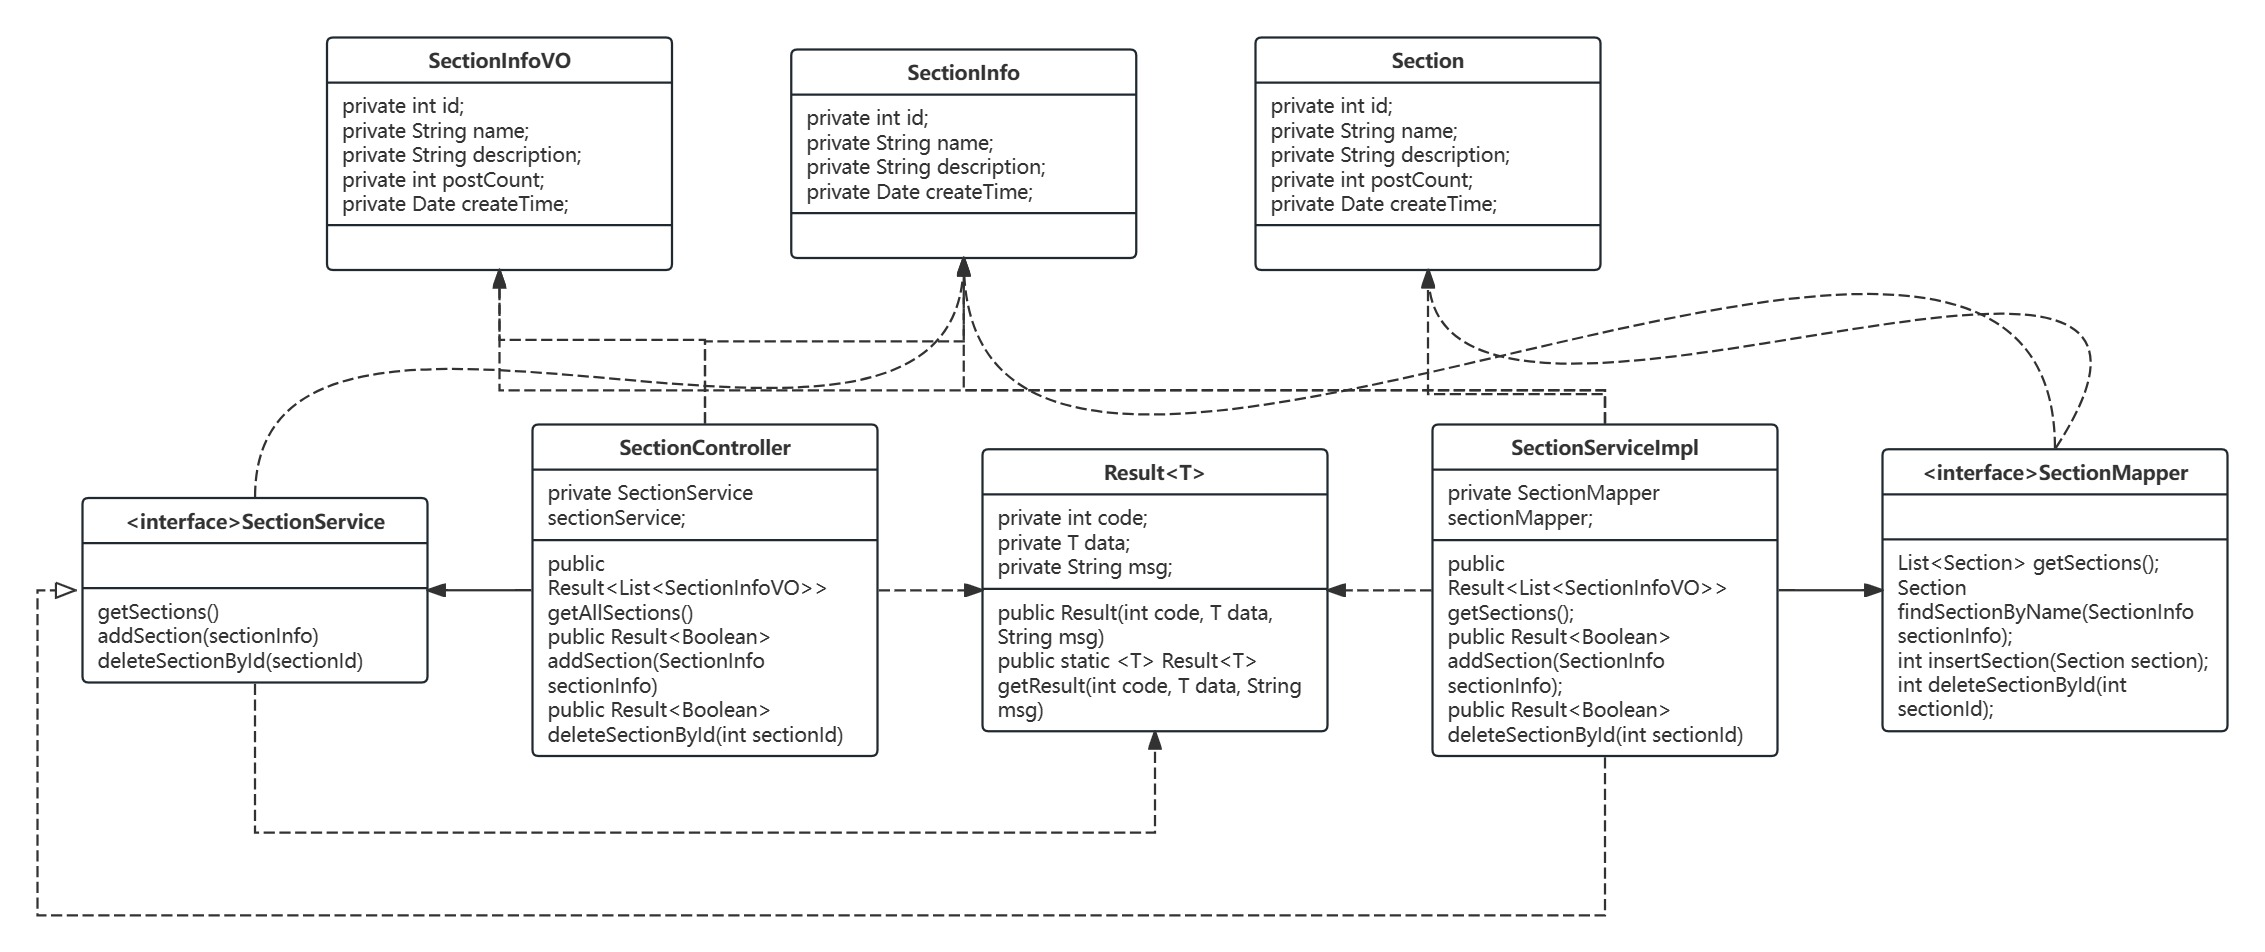
\includegraphics[scale=0.2]{精化类模型图/section.jpg}
  \caption{模块管理类图}
\end{figure}

\subsubsubsection{模块管理时序图}

\begin{figure}[H]
  \centering
  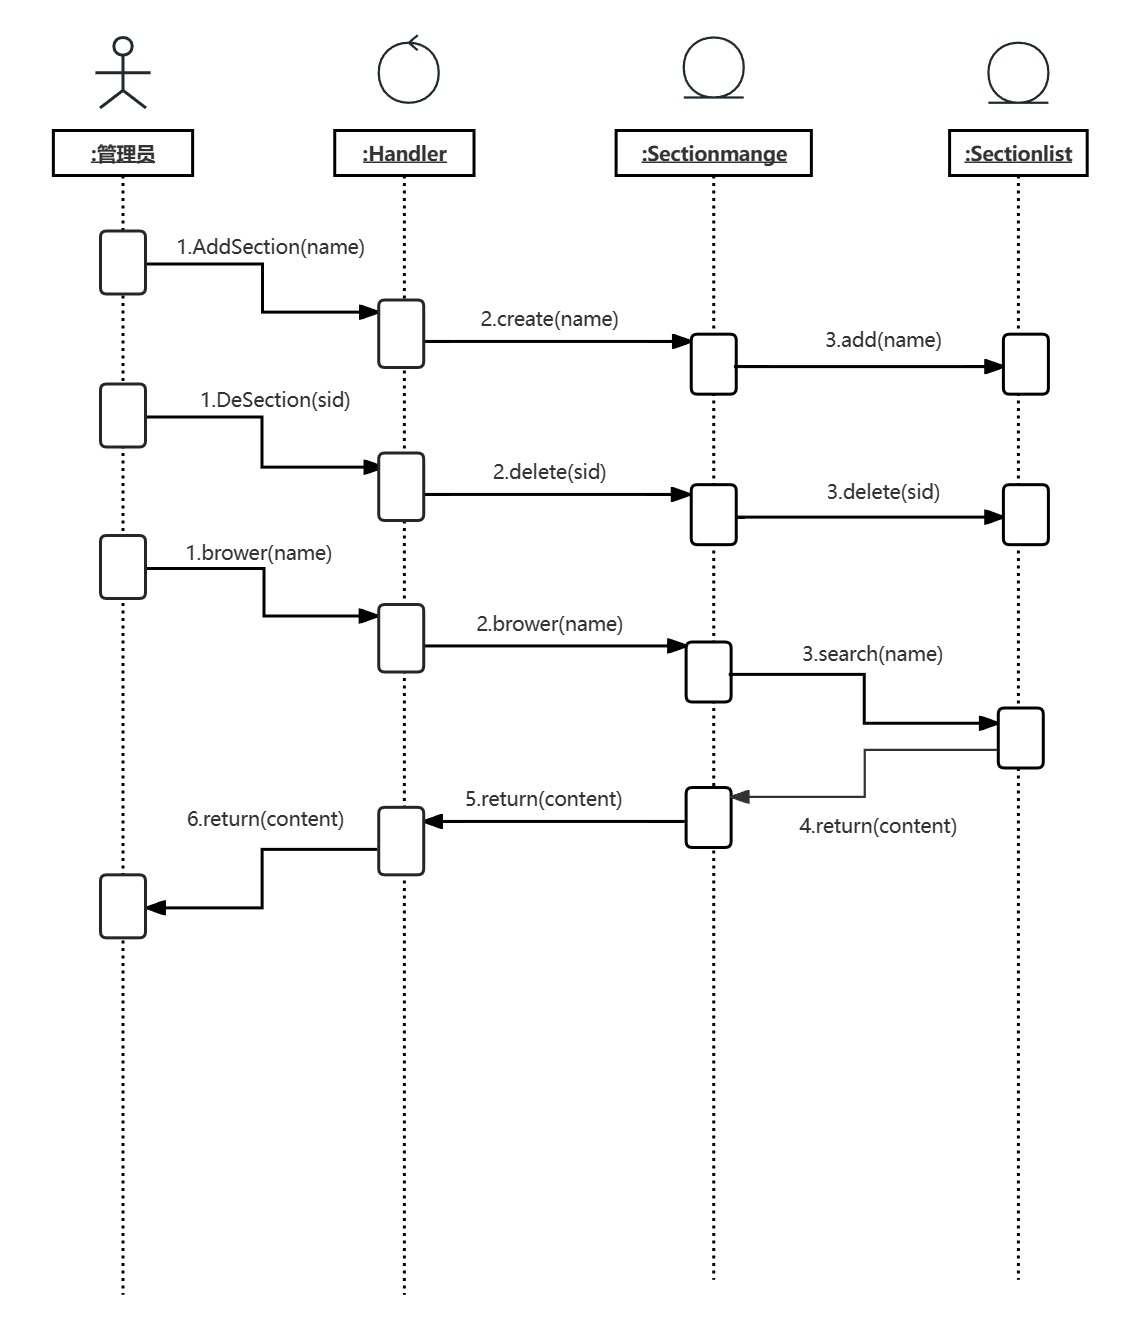
\includegraphics[scale=0.3]{顺序图/管理员版块管理.png}
  \caption{管理员管理版块}
\end{figure}



\newpage

\subsection{界面设计}

\subsubsection{用户登录}

\begin{figure}[H]
  \centering
  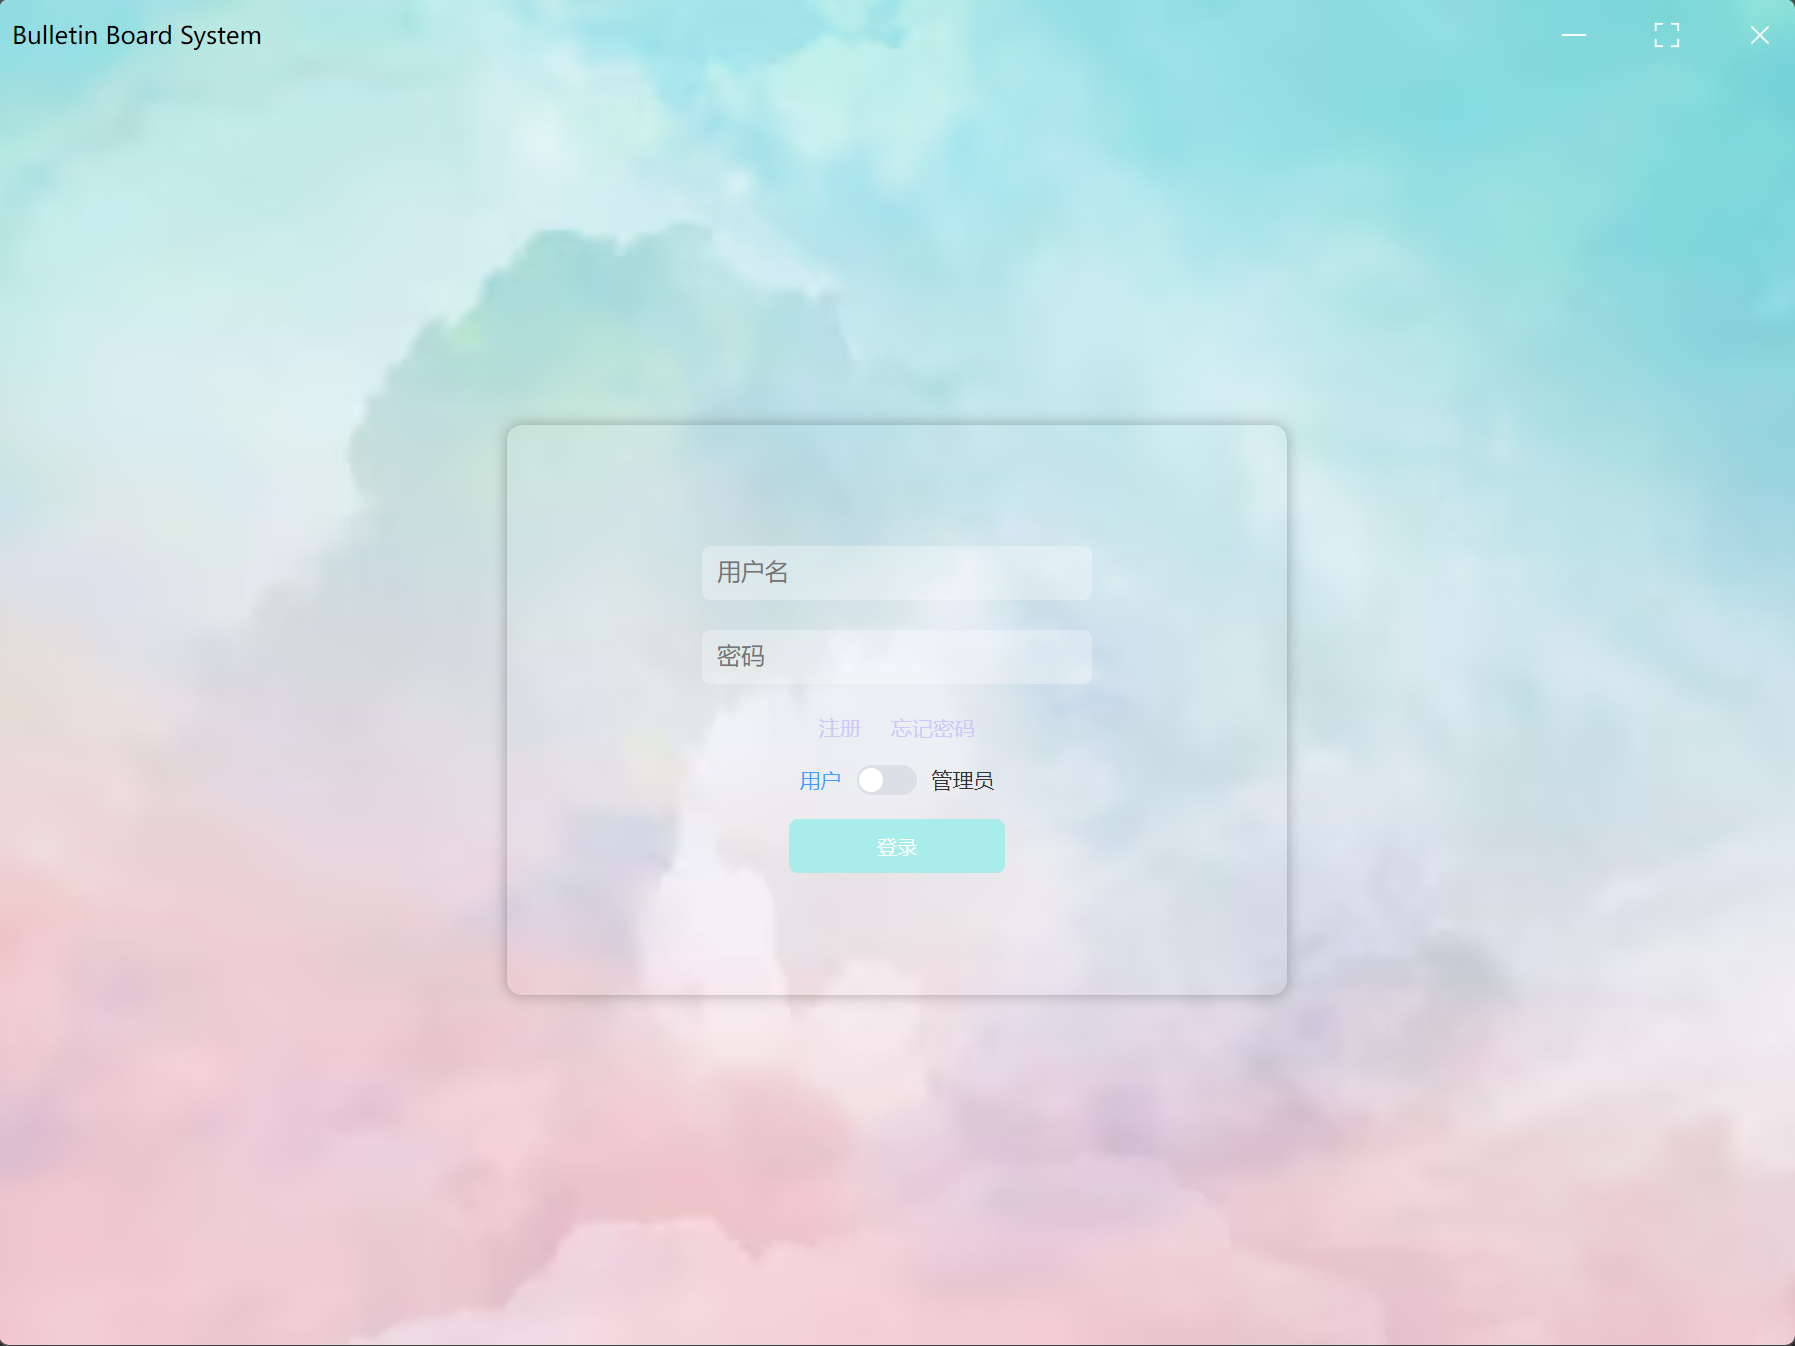
\includegraphics[scale=0.3]{系统实现/登录.png}
  \caption{用户登录界面}
\end{figure}

\subsubsection{用户注册}

\begin{figure}[H]
  \centering
  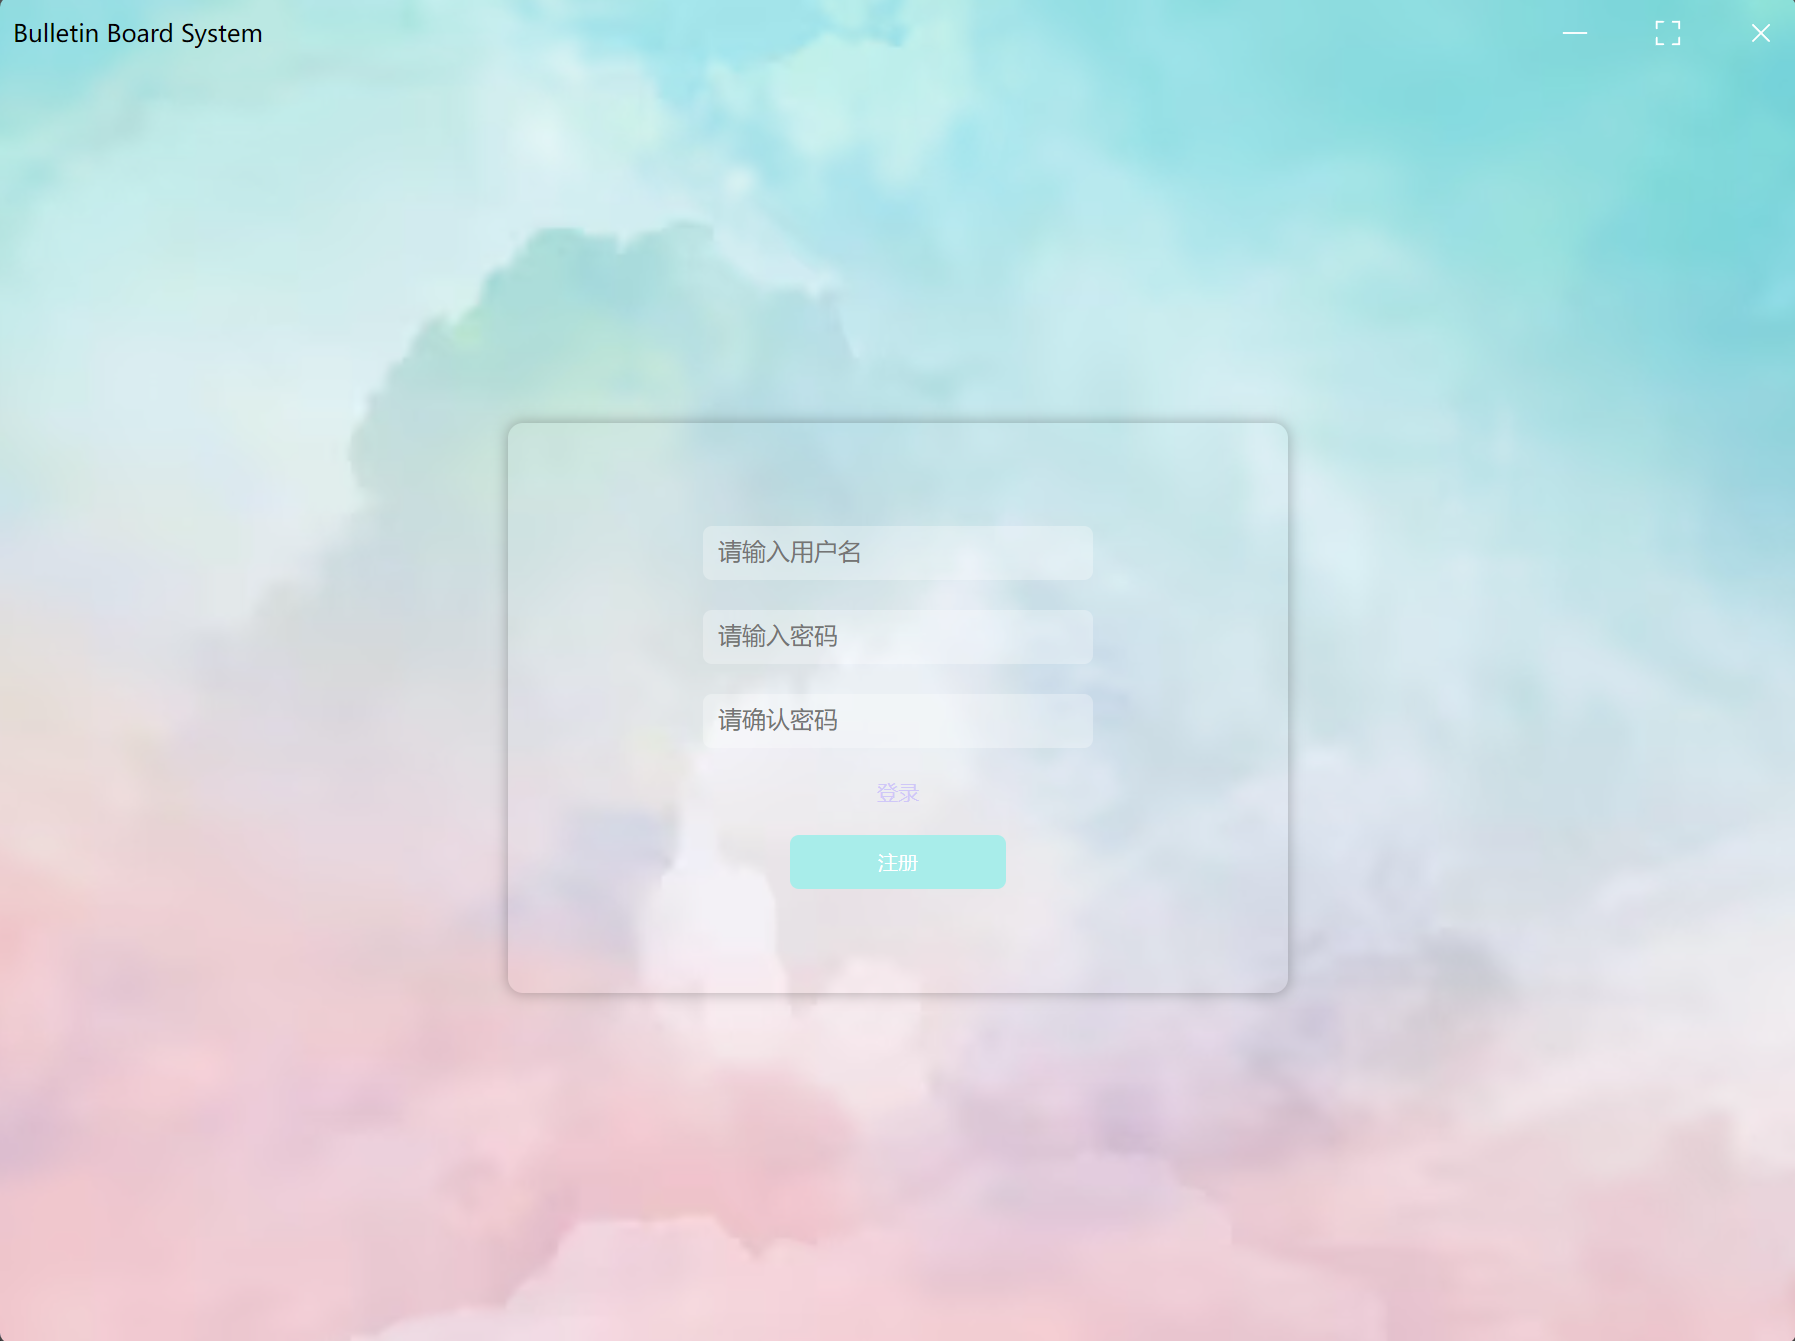
\includegraphics[scale=0.3]{系统实现/注册.png}
  \caption{用户注册界面}
\end{figure}

\subsubsection{帖子界面}

\begin{figure}[H]
  \centering
  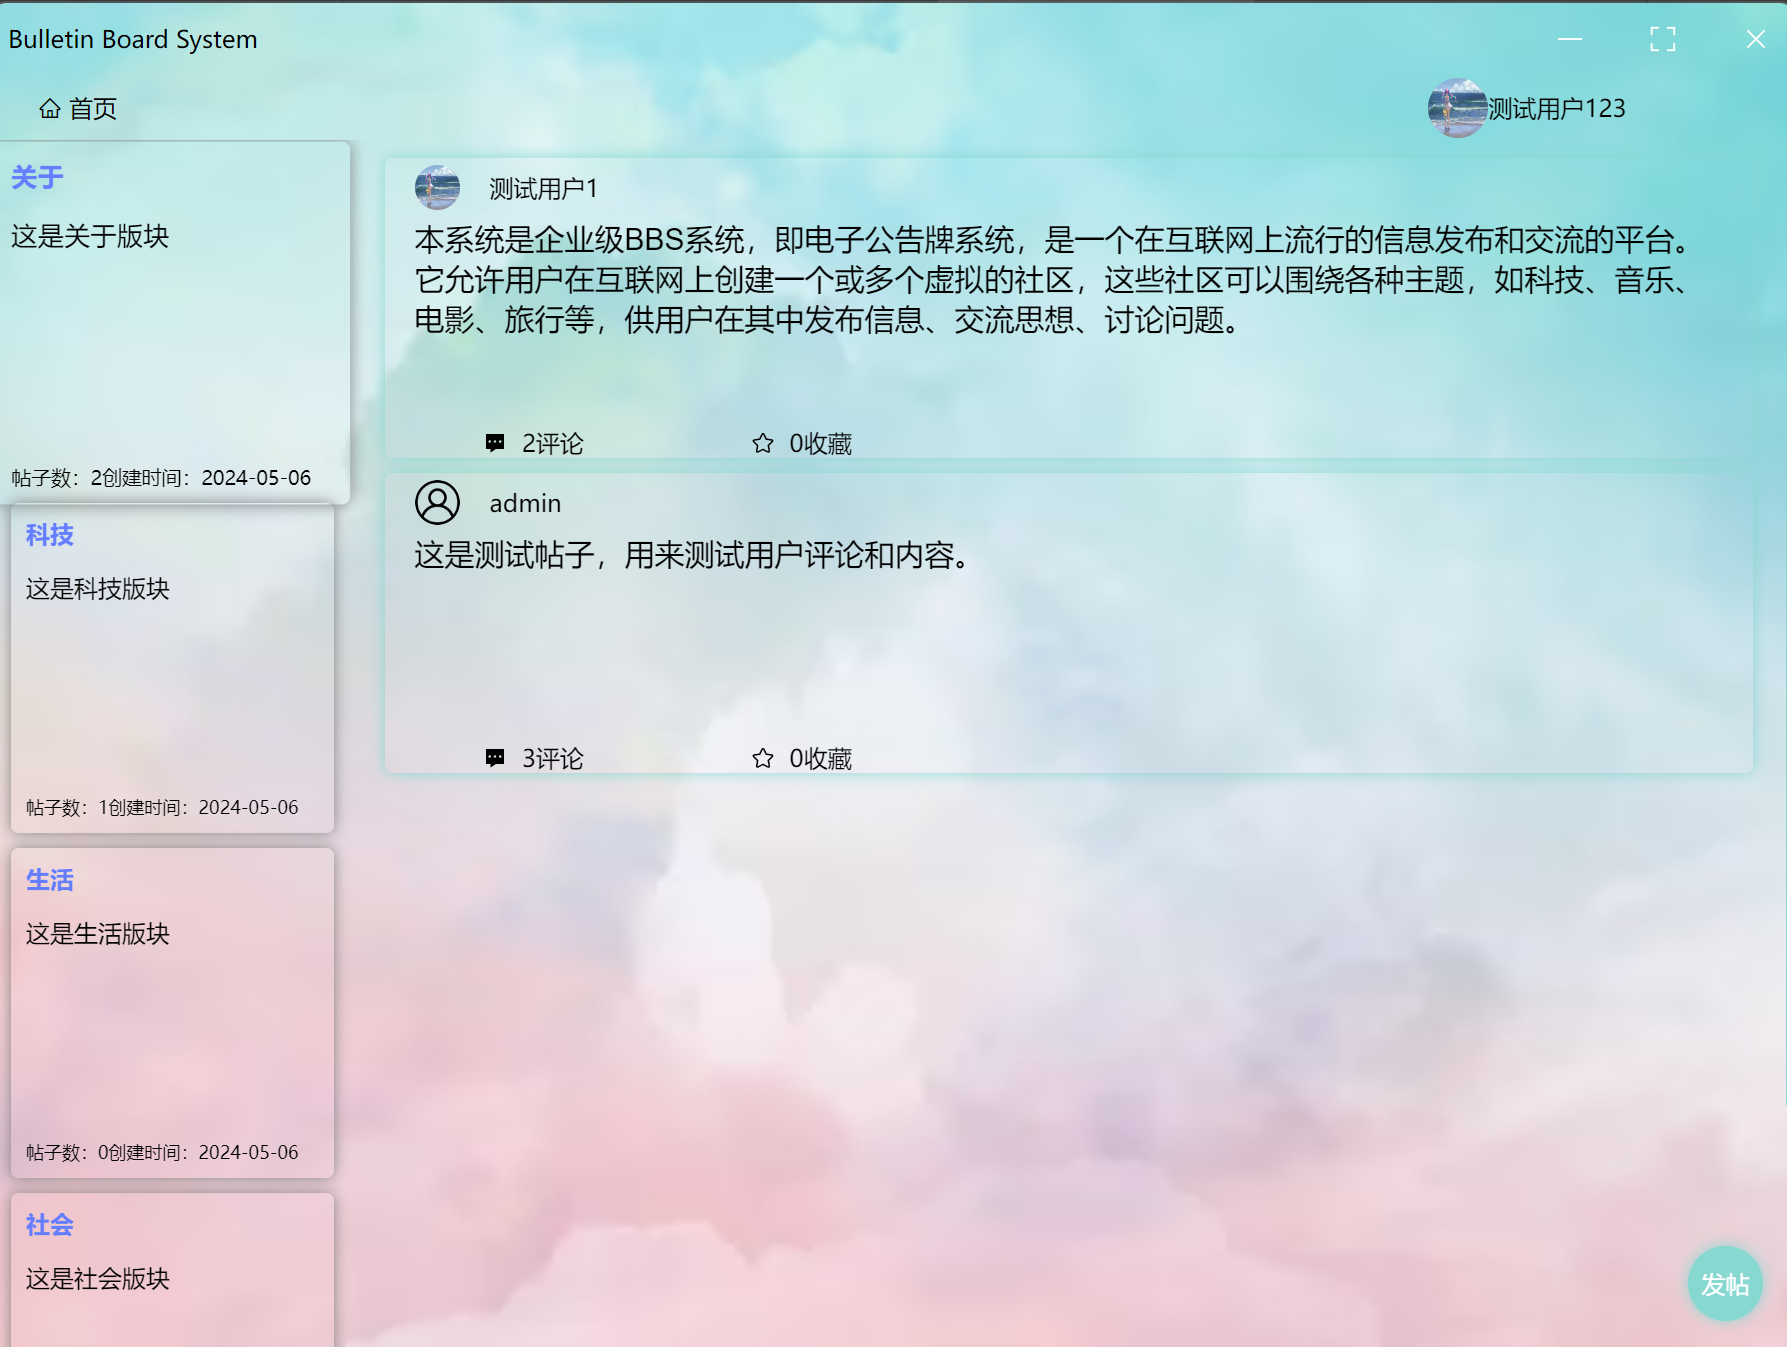
\includegraphics[scale=0.3]{系统实现/用户帖子.png}
  \caption{帖子界面}
\end{figure}

\begin{figure}[H]
  \centering
  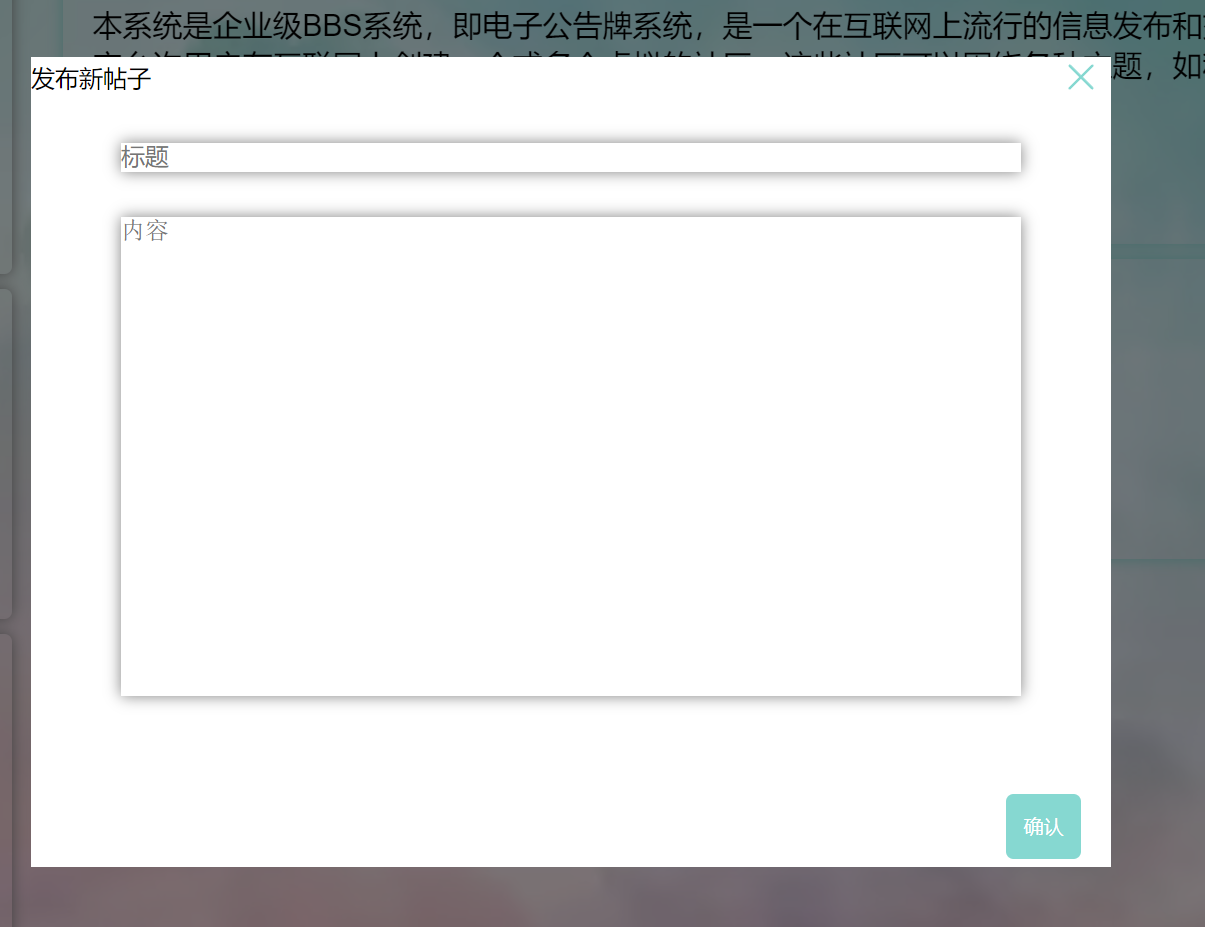
\includegraphics[scale=0.3]{系统实现/发布帖子.png}
  \caption{发布帖子界面}
\end{figure}

\subsubsection{评论界面}

\begin{figure}[H]
  \centering
  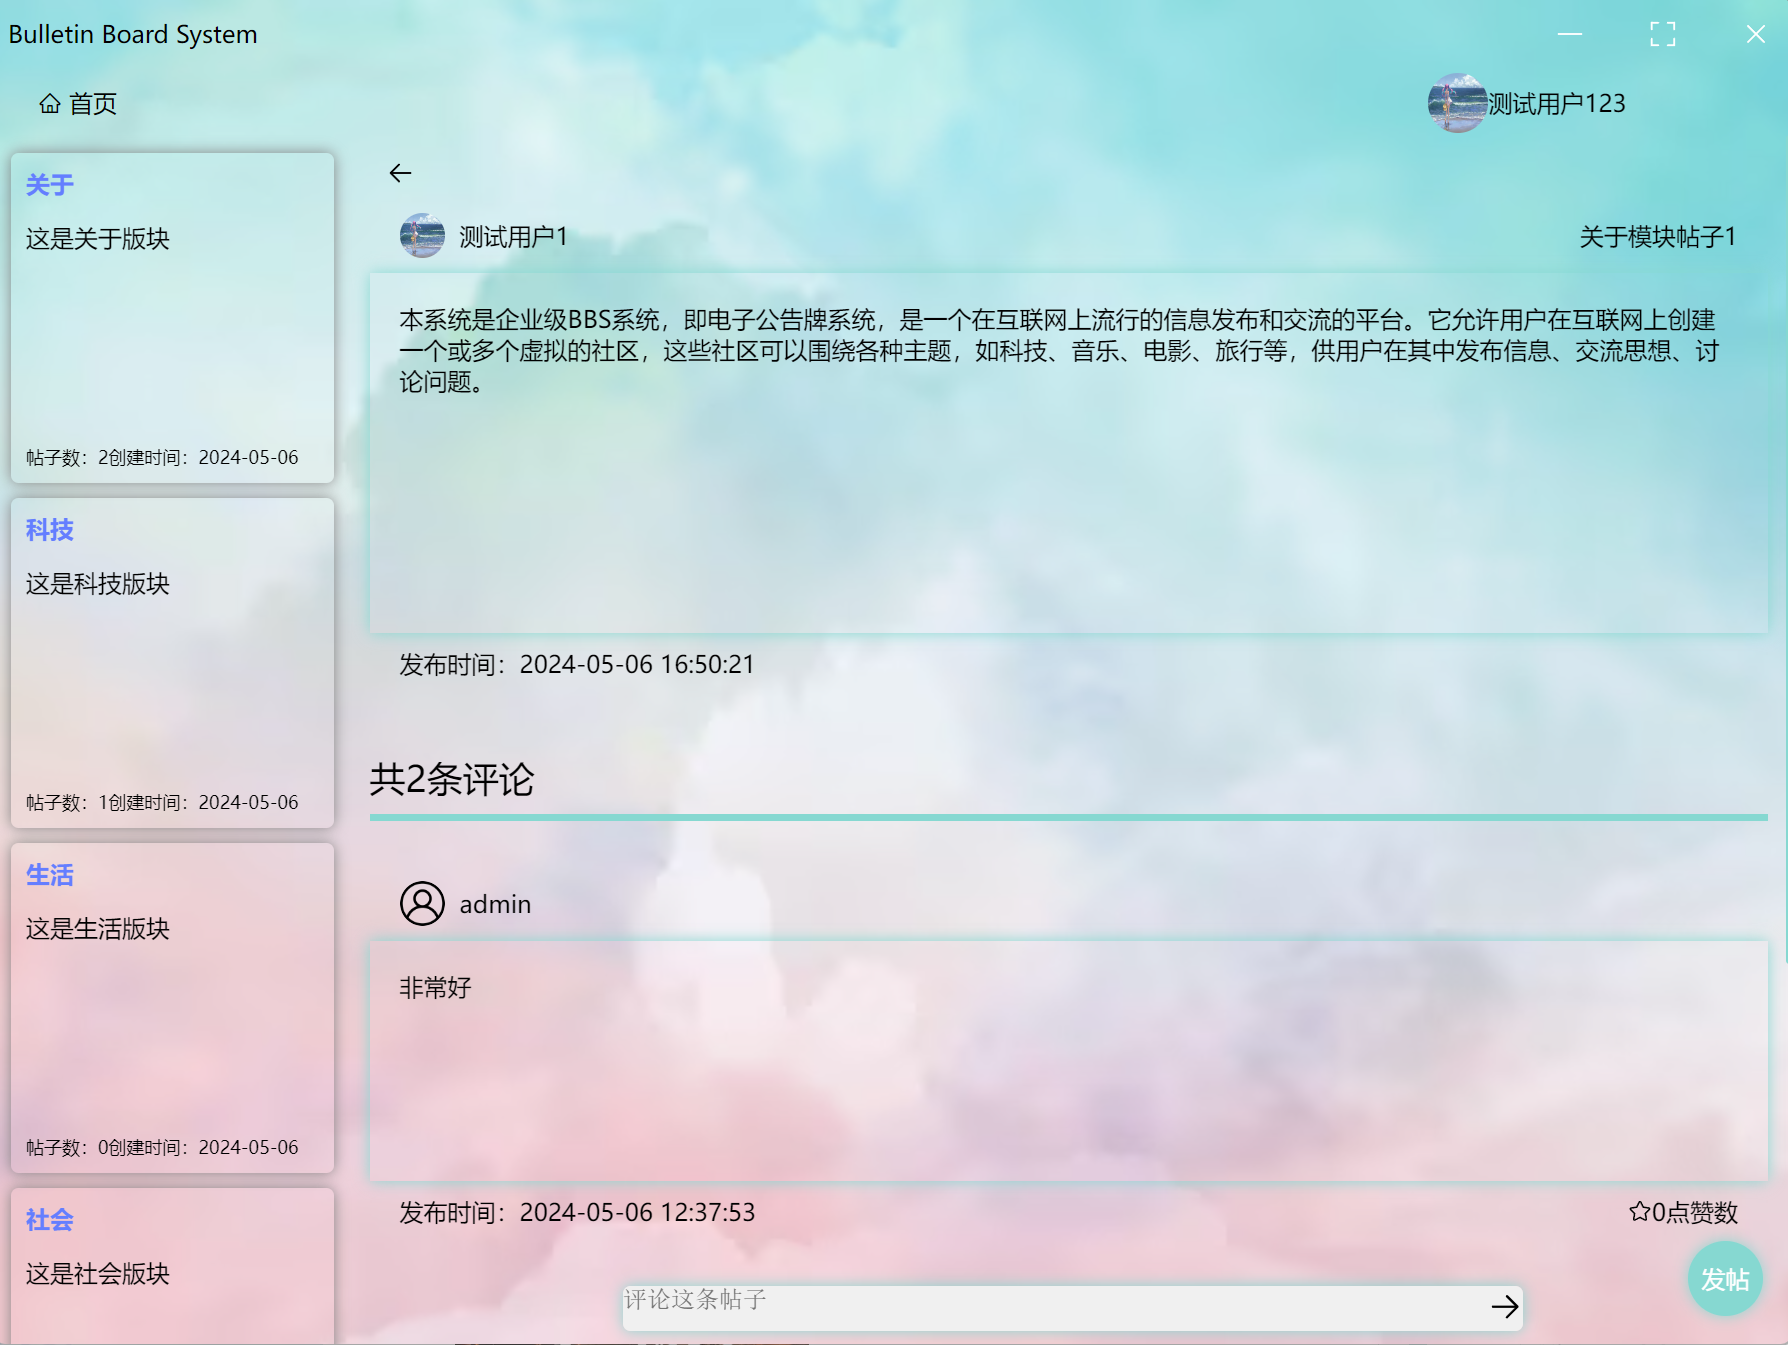
\includegraphics[scale=0.3]{系统实现/帖子页面和评论.png}
  \caption{评论界面}
\end{figure}


\subsubsection{管理员界面}

\begin{figure}[H]
  \centering
  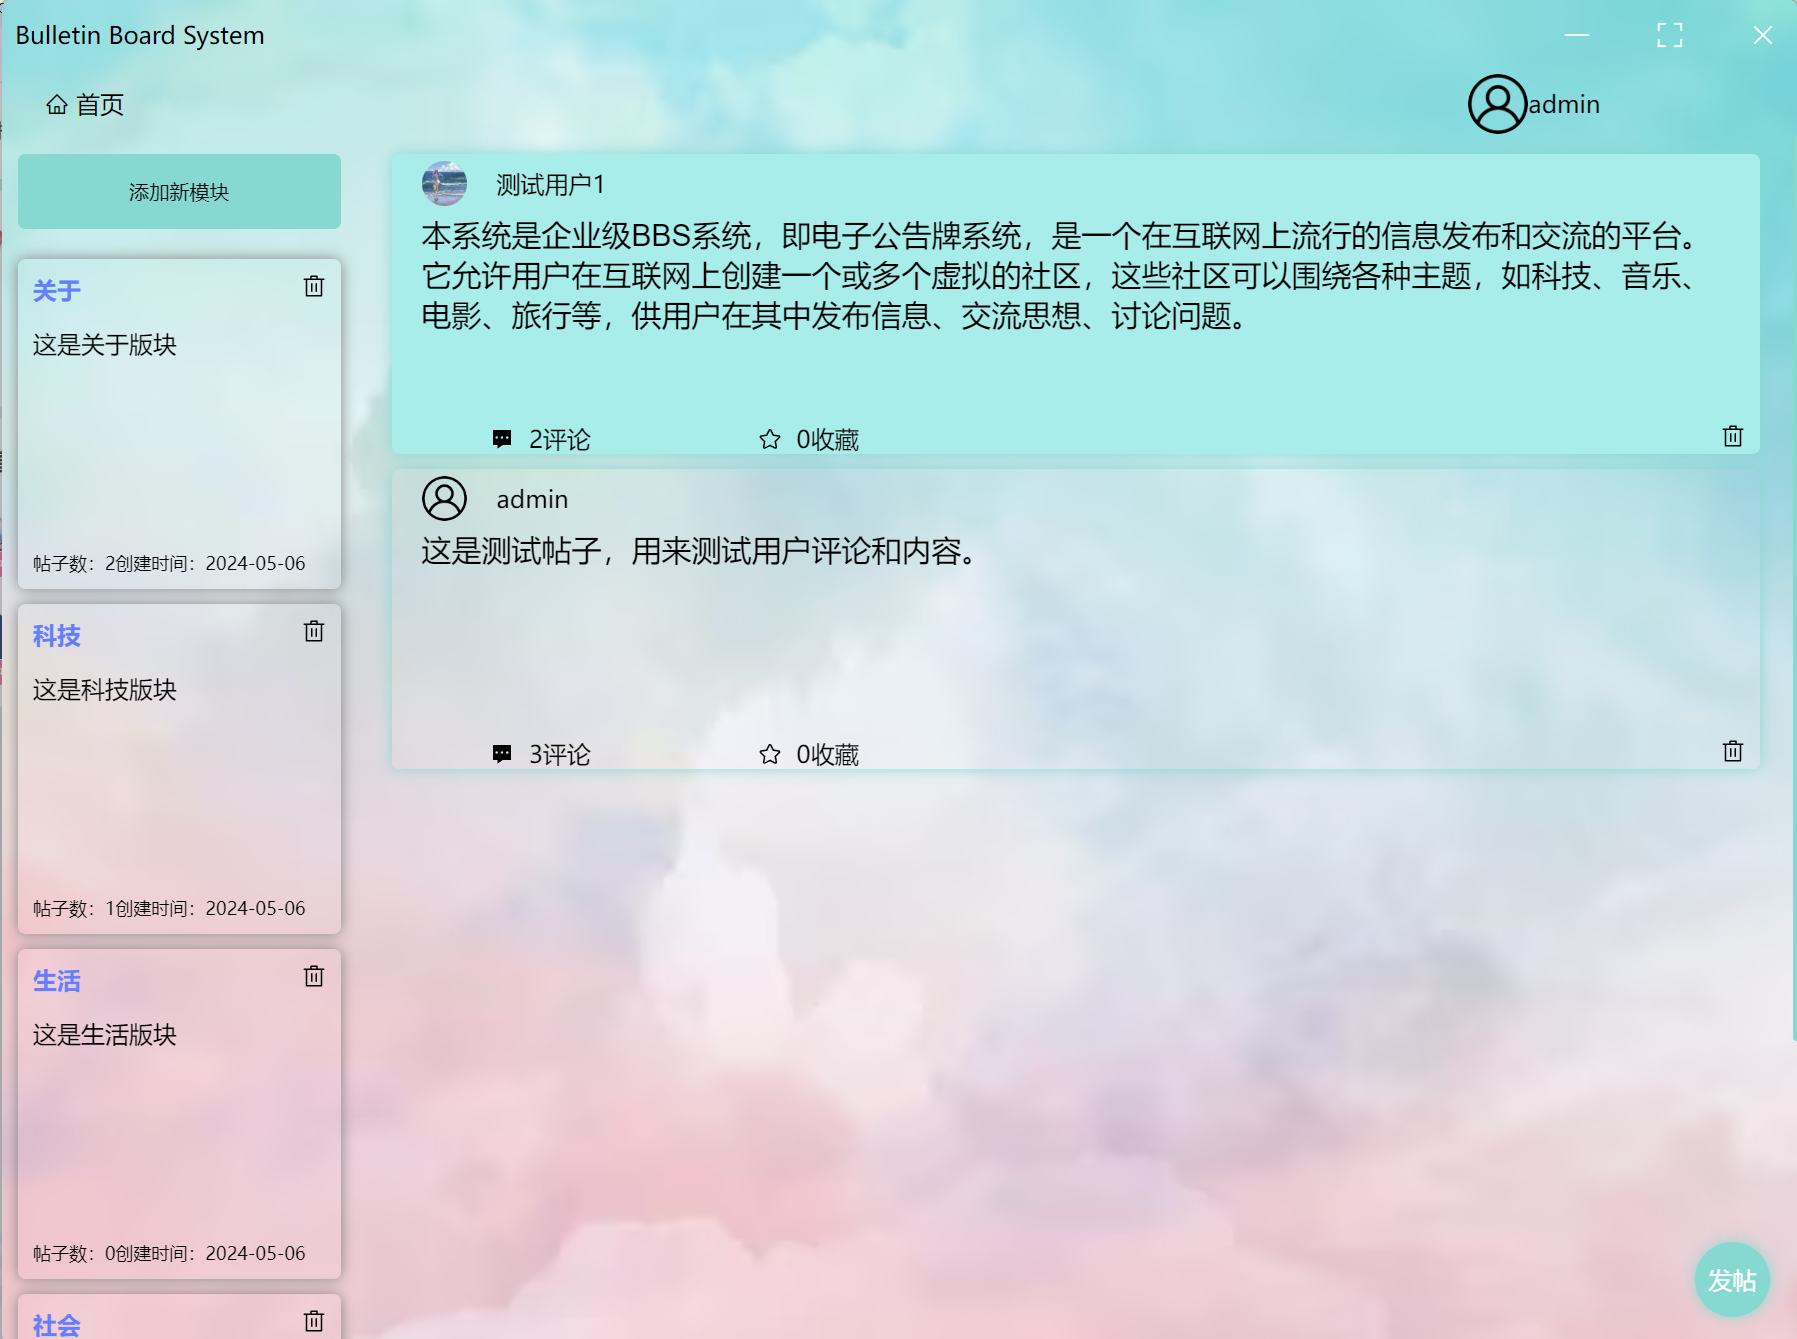
\includegraphics[scale=0.3]{系统实现/管理员界面.png}
  \caption{管理员界面}
\end{figure}






\newpage
\subsection{非功能设计}
\subsubsection{性能需求}
\begin{enumerate}
  \item 响应时间: 系统应该快速响应用户请求,确保快速加载图片和数据。
  \item 并发处理: 系统需要支持多用户并发访问,确保稳定的性能。
  \item 扩展性: 能够在需要时扩展系统以处理更多用户和数据。
\end{enumerate}

\subsubsection{安全性需求}
\begin{enumerate}
  \item 身份验证和授权: 用户应该通过身份验证访问系统,并根据角色获得适当的权限。
  \item 数据保护: 图片和用户数据应该加密存储,以防止未经授权的访问。
\end{enumerate}

\subsubsection{可靠性需求}
\begin{enumerate}
  \item 系统应该可靠,最小化系统宕机或故障的时间。
\end{enumerate}

\subsubsection{可用性需求}
\begin{enumerate}
  \item 界面设计:采取直观的界面设计,以便用户能够轻松地使用系统。
  \item 性能优化:确保快速加载图片和页面,以减少用户等待时间。 
\end{enumerate}

\subsubsection{可维护性需求}
\begin{enumerate}
  \item 代码可读性:项目代码应该写好注释,以便维护和团队合作。
  \item 错误日志和监控:保存系统的错误和异常情况和系统日志
\end{enumerate}

\subsubsection{可拓展性需求}
\begin{enumerate}
  \item 模块化设计:将系统设计成模块化的,以便能够添加新功能或组件。
\end{enumerate}




\newpage
\section{数据库设计}

\subsection{逻辑建模}

\begin{figure}[H]
  \centering
  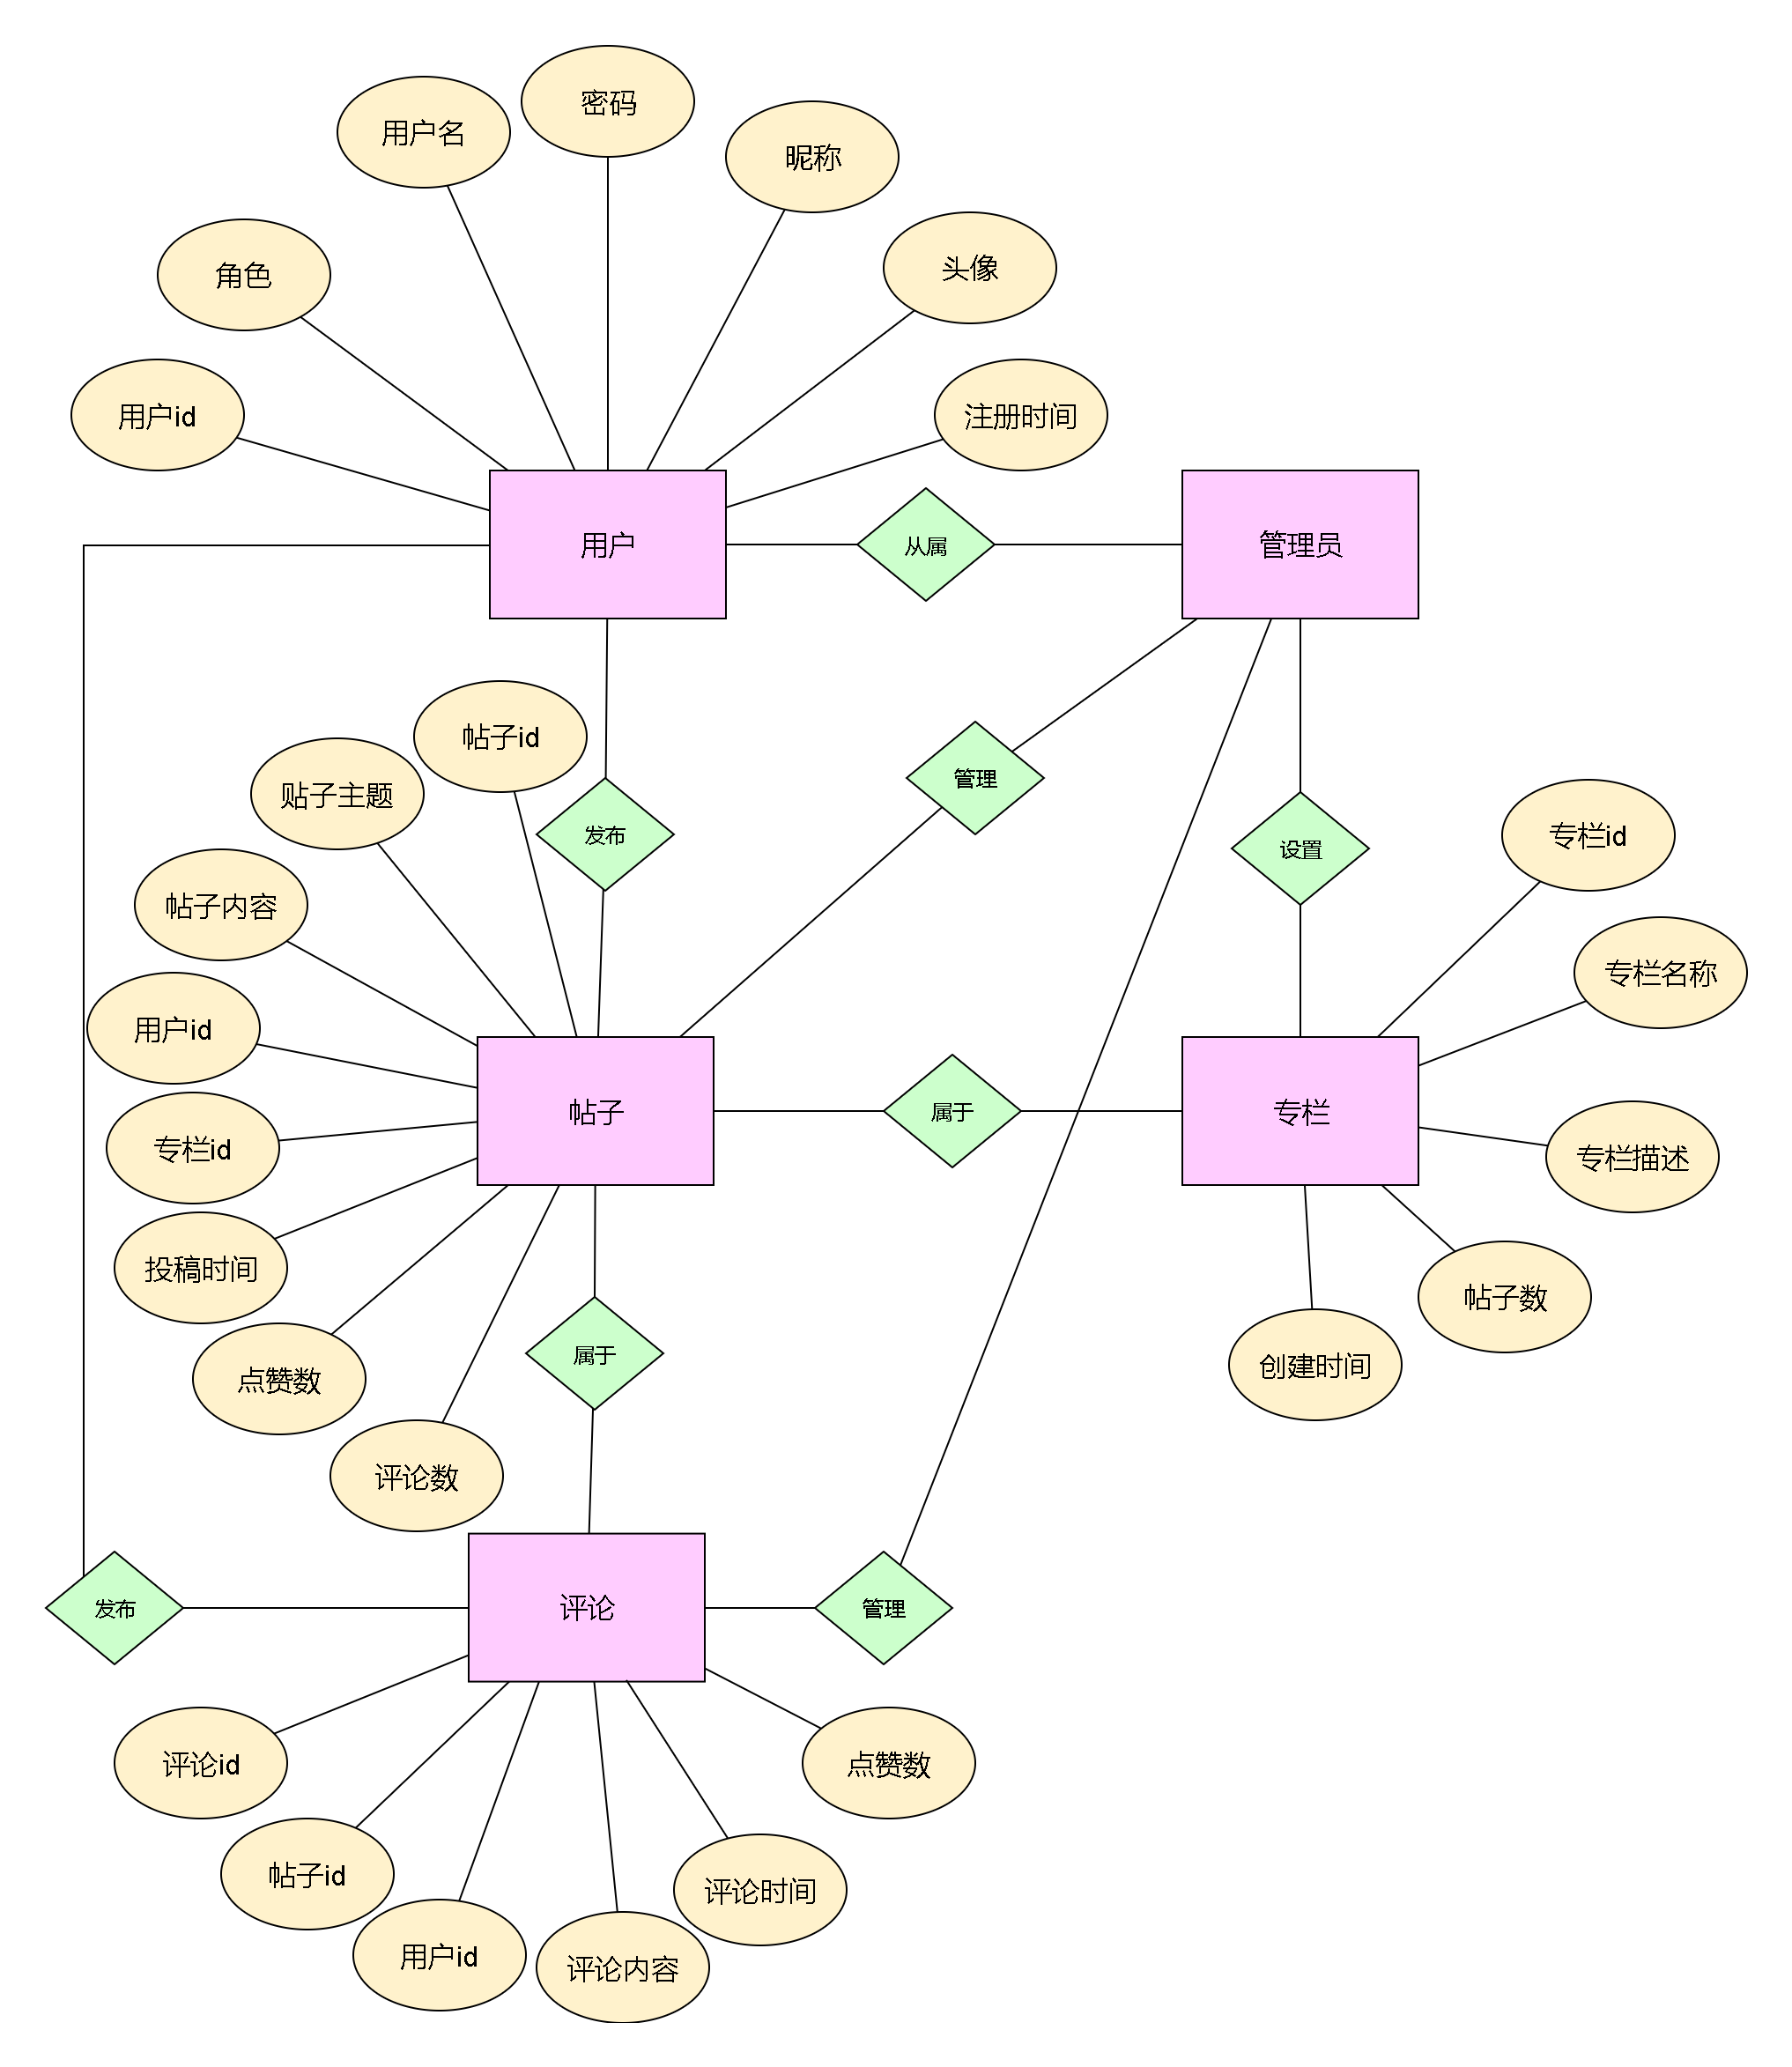
\includegraphics[scale=0.2]{数据库部分/bbs-ER图.jpg}
  \caption{ER图}
\end{figure}


\subsection{数据库设计}

\subsubsection{用户表}

\begin{table}[H]
  \centering
  \begin{tabular}{|c|c|c|c|c|c|}
  \hline
      字段名 & 类型 & 长度 & 是否可为空&备注&含义\\ \hline
      id & int & - & 否 & 主键 & 用户id \\ \hline
      role & varchar &255  & 否 &  & 用户角色 \\ \hline
      username & varchar &255  & 否 &  & 用户名 \\ \hline
      password & varchar & 255 & 否 &  & 密码 \\ \hline
      nickname & varchar & 255 & 是 &  & 昵称 \\ \hline
      avatar & varchar & 255 & 是 &  & 头像 \\ \hline
      registerTime & datetime &-  & 否 &  & 注册时间 \\ \hline
  \end{tabular}
  \caption{用户表}
\end{table}

\subsubsection{帖子表}

\begin{table}[H]
  \centering
  \begin{tabular}{|c|c|c|c|c|c|}
  \hline
      字段名 & 类型 & 长度 & 是否可为空&备注&含义\\ \hline
      id & int & - & 否 & 主键 & 帖子id \\ \hline
      title & varchar &255  & 否 &  & 标题 \\ \hline
      content & text & - & 否 &  & 内容 \\ \hline
      uid & int & - & 否 & 外键 & 用户id \\ \hline
      sid & int & - & 否 & 外键 & 模块id \\ \hline
      postedTime & datetime & - & 否 &  & 创建时间 \\ \hline
      like\_count & int & - & 否 &  & 点赞数 \\ \hline
      comment\_count & int & - & 否 &  & 评论数 \\ \hline
  \end{tabular}
  \caption{帖子表}
\end{table}

\subsubsection{评论表}

\begin{table}[H]
  \centering
  \begin{tabular}{|c|c|c|c|c|c|}
  \hline
      字段名 & 类型 & 长度 & 是否可为空&备注&含义\\ \hline
      id & int & - & 否 & 主键 & 评论id \\ \hline
      content & text & - & 否 &  & 内容 \\ \hline
      uid & int & - & 否 & 外键 & 用户id \\ \hline
      pid & int & - & 否 & 外键 & 帖子id \\ \hline
      commentTime & datetime &-  & 否 &  & 评论时间 \\ \hline
      like\_count & int &-  & 否 &  & 点赞数 \\ \hline
  \end{tabular}
  \caption{评论表}
\end{table}

\subsubsection{模块表}

\begin{table}[H]
  \centering
  \begin{tabular}{|c|c|c|c|c|c|}
  \hline
      字段名 & 类型 & 长度 & 是否可为空&备注&含义\\ \hline
      id & int & - & 否 & 主键 & 模块id \\ \hline
      name & varchar &255  & 否 &  & 模块名 \\ \hline
      description & text & - & 否 &  & 描述 \\ \hline
      post\_count & int & - & 否 &  & 帖子数 \\ \hline
      createTime & datetime & - & 否 &  & 创建时间 \\ \hline
  \end{tabular}
  \caption{模块表}
\end{table}



\newpage
\section{系统实现}
\subsection{系统配置}

\textbf{本项目使用的开发环境如下:}
\begin{itemize}
  \item 操作系统:Windows 11
  \item 项目架构:前后端分离,前端使用vue框架,后端使用SpringBoot框架
  \item 开发工具:IntelliJ IDEA 、WebStorm、Visual Studio Code
  \item 开发语言:Java、vue、JavaScript、HTML、CSS、SQL
  \item 数据库:MySQL
  \item 版本控制:Git
  \item 项目管理:Maven
\end{itemize}


\textbf{前端项目部署在本地5173端口}

\begin{figure}[H]
  \centering
  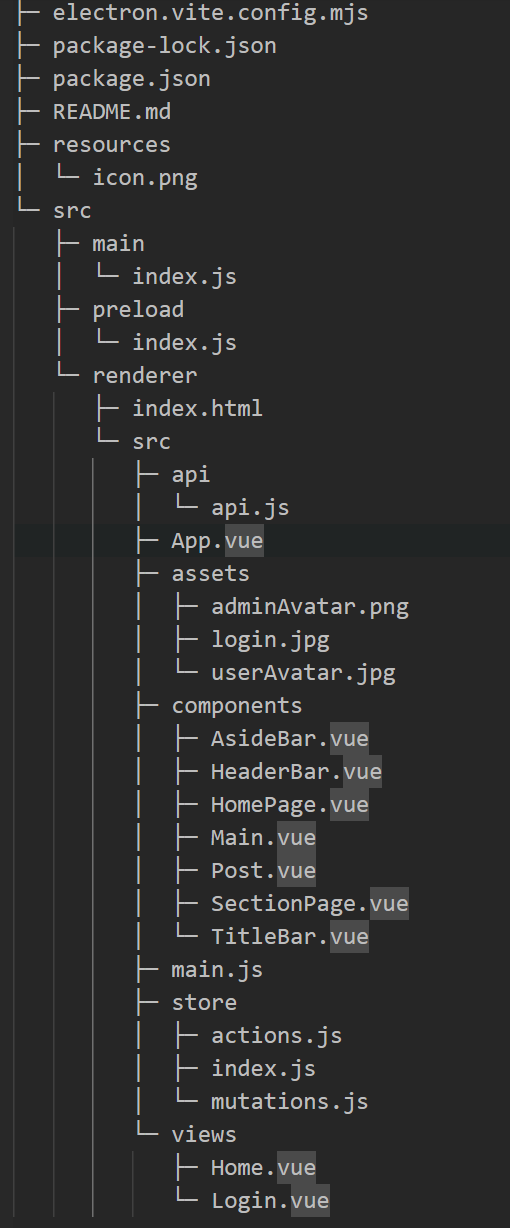
\includegraphics[scale=0.3]{系统实现/前端项目结构.png}
  \caption{前端项目结构}
\end{figure}

\textbf{后端项目部署在本地8080端口}

\begin{figure}[H]
  \centering
  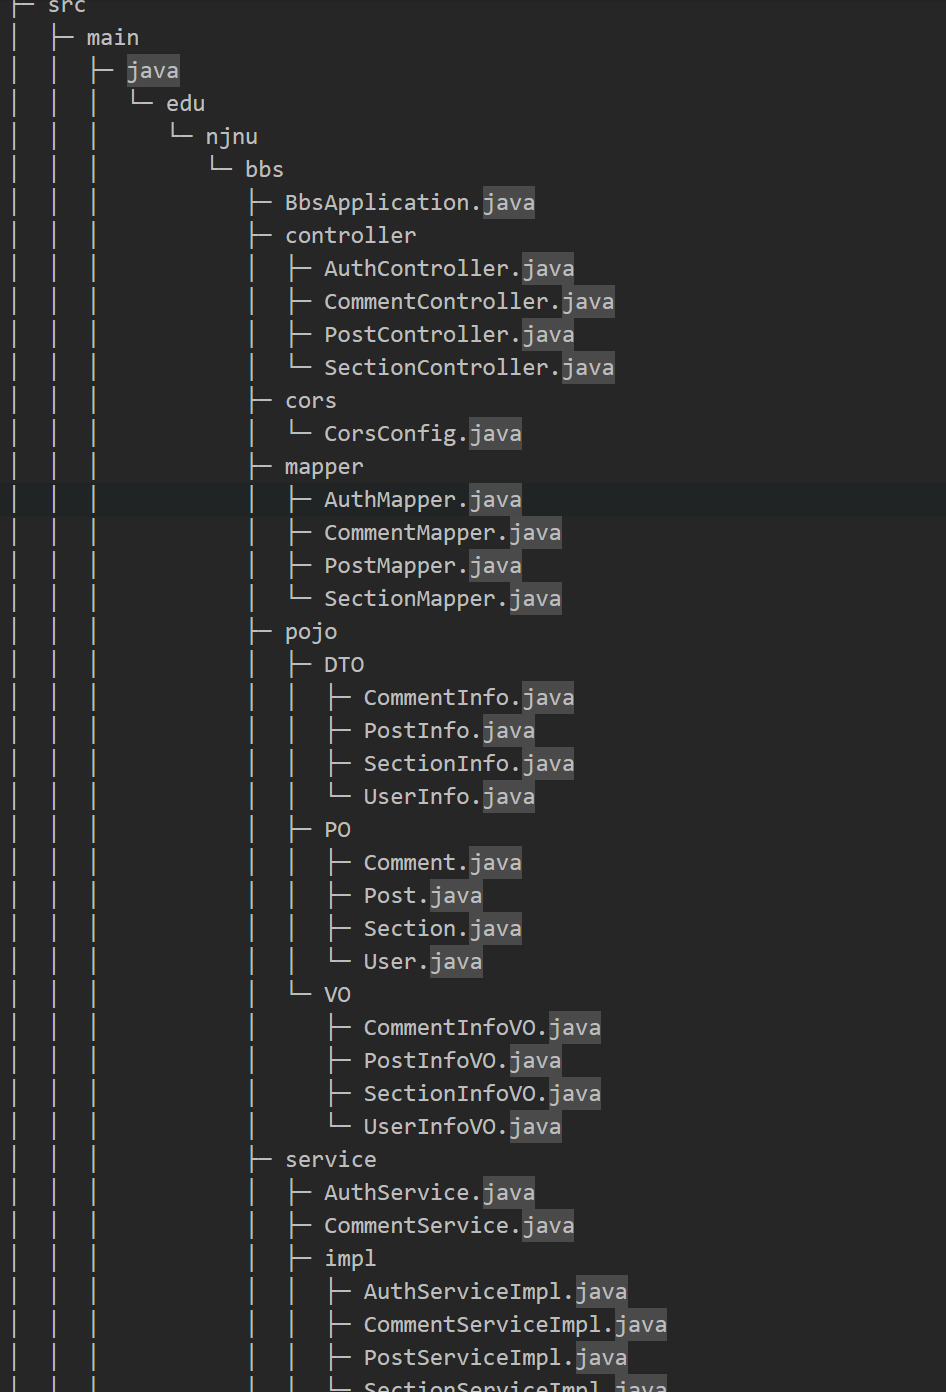
\includegraphics[scale=0.3]{系统实现/后端项目结构.png}
  \caption{后端项目结构}
\end{figure}


\subsection{系统主页面}

\begin{figure}[H]
  \centering
  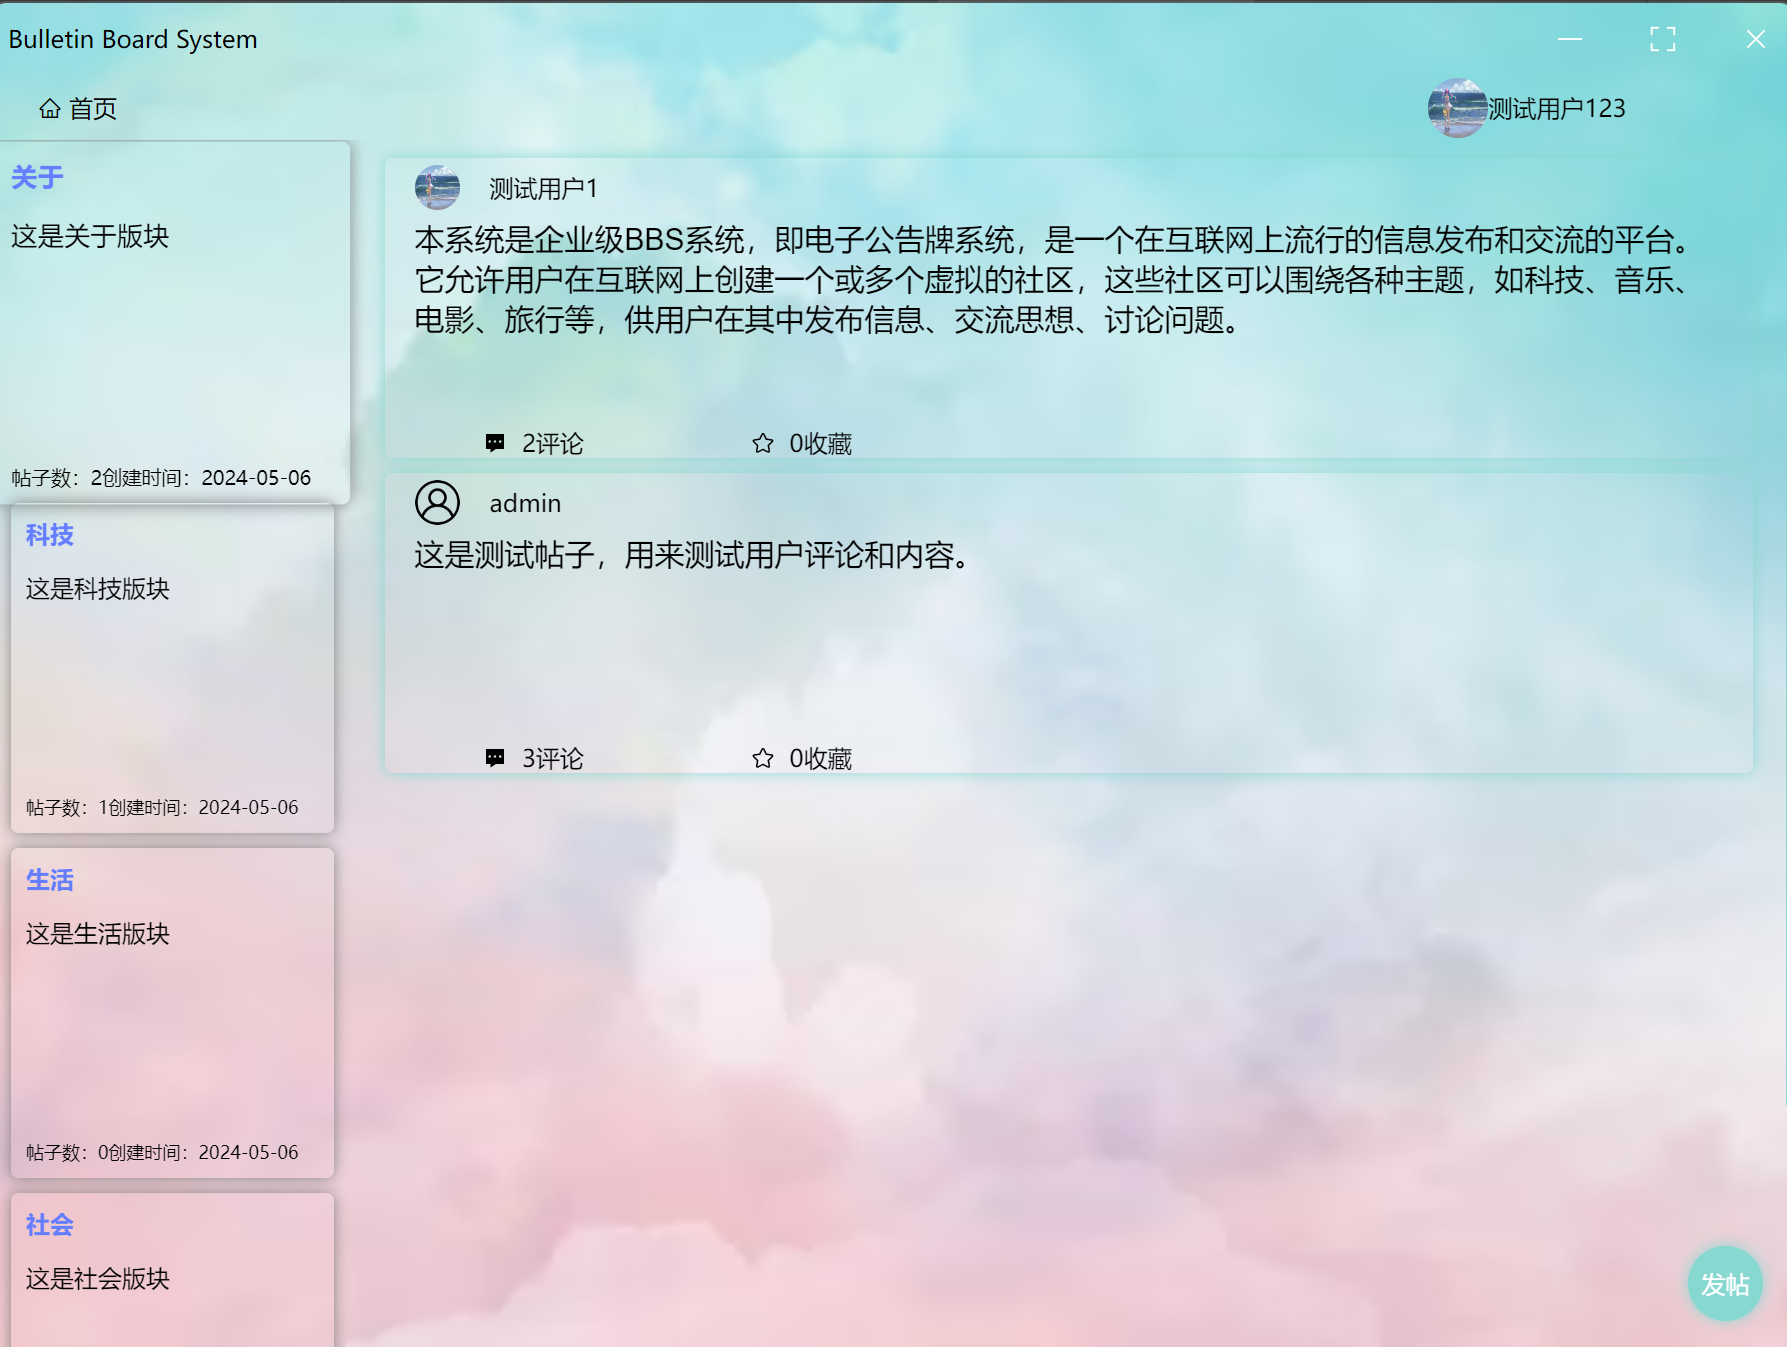
\includegraphics[scale=0.3]{系统实现/用户帖子.png}
  \caption{系统主页面}
\end{figure}



\subsection{系统功能实现}

\subsubsection{账号管理功能实现}

\begin{figure}[H]
  \centering
  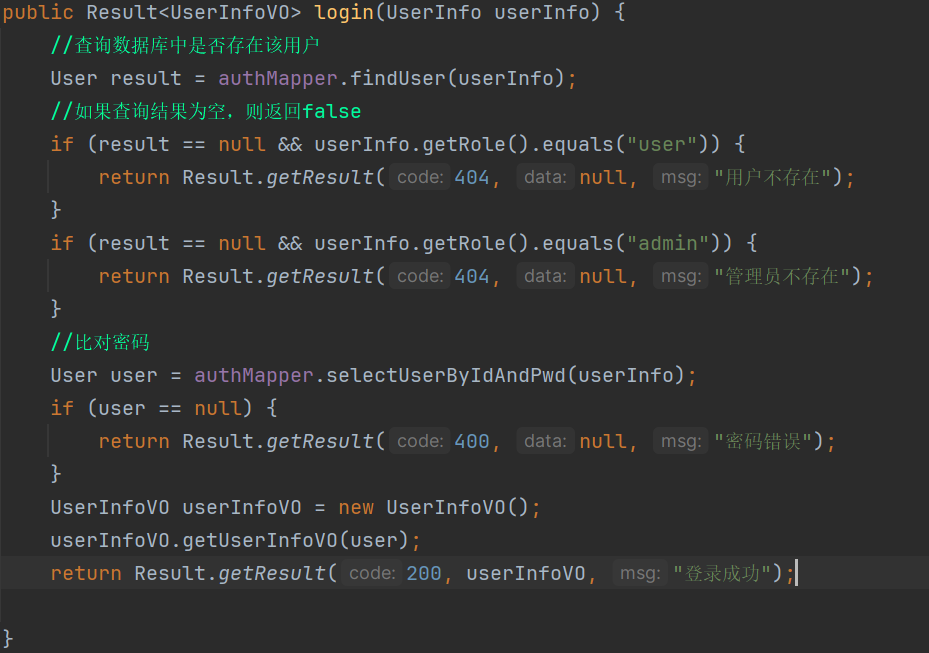
\includegraphics[scale=0.3]{系统实现/账户管理实现.png}
  \caption{账号管理功能实现}
\end{figure}

\subsubsection{帖子管理功能实现}

\begin{figure}[H]
  \centering
  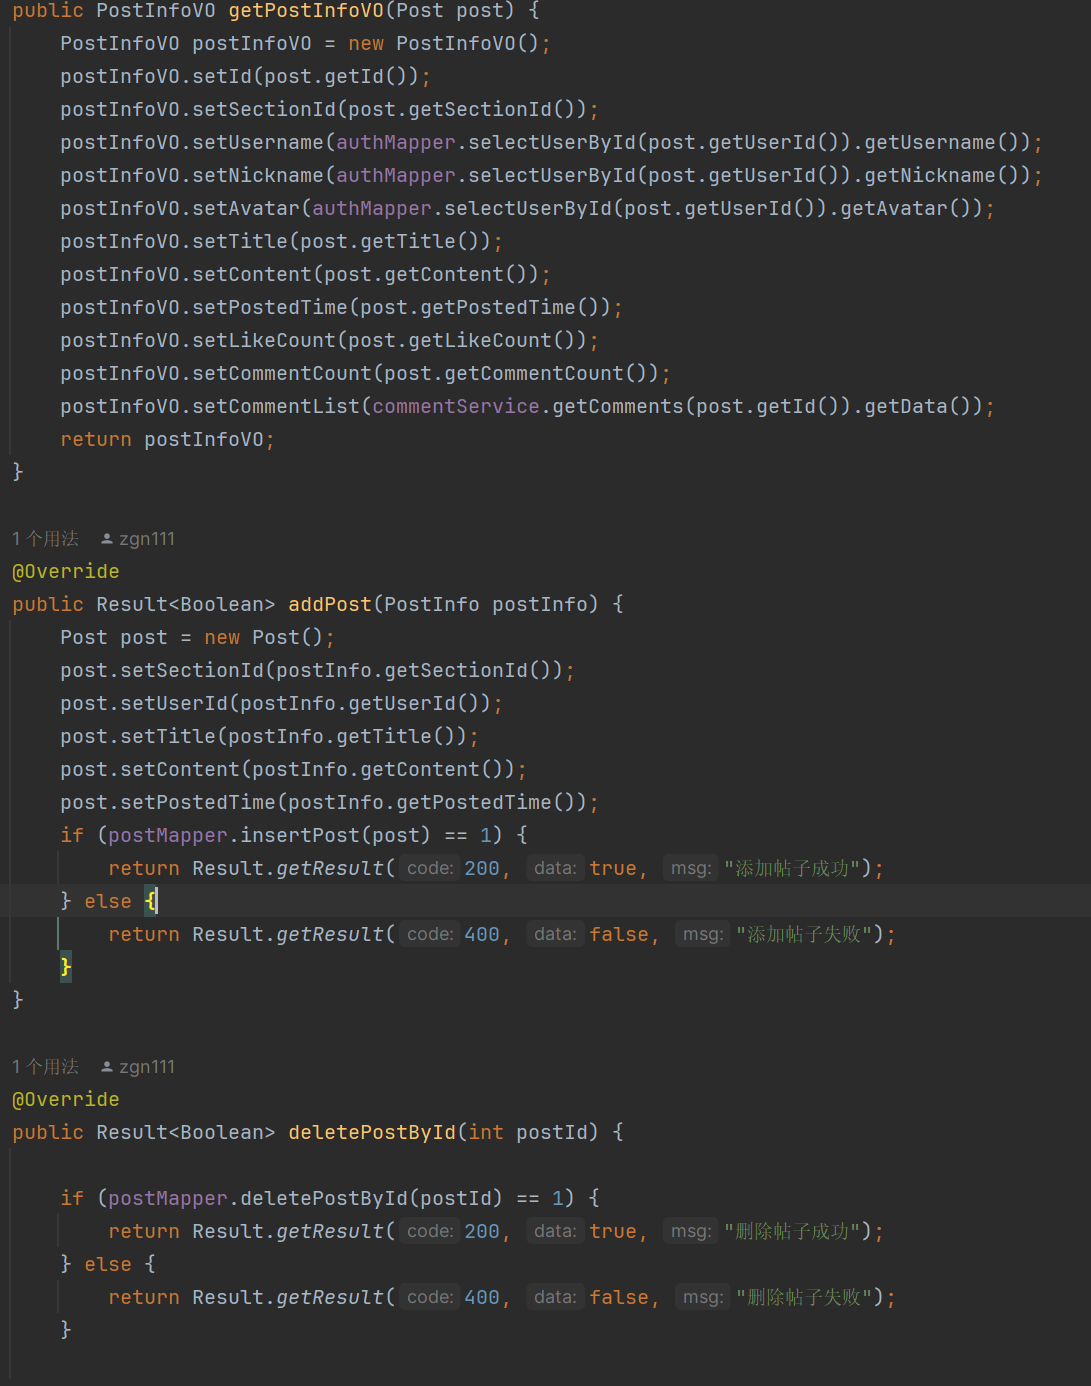
\includegraphics[scale=0.3]{系统实现/帖子功能实现.png}
  \caption{帖子管理功能实现}
\end{figure}

\subsubsection{评论管理功能实现}

\begin{figure}[H]
  \centering
  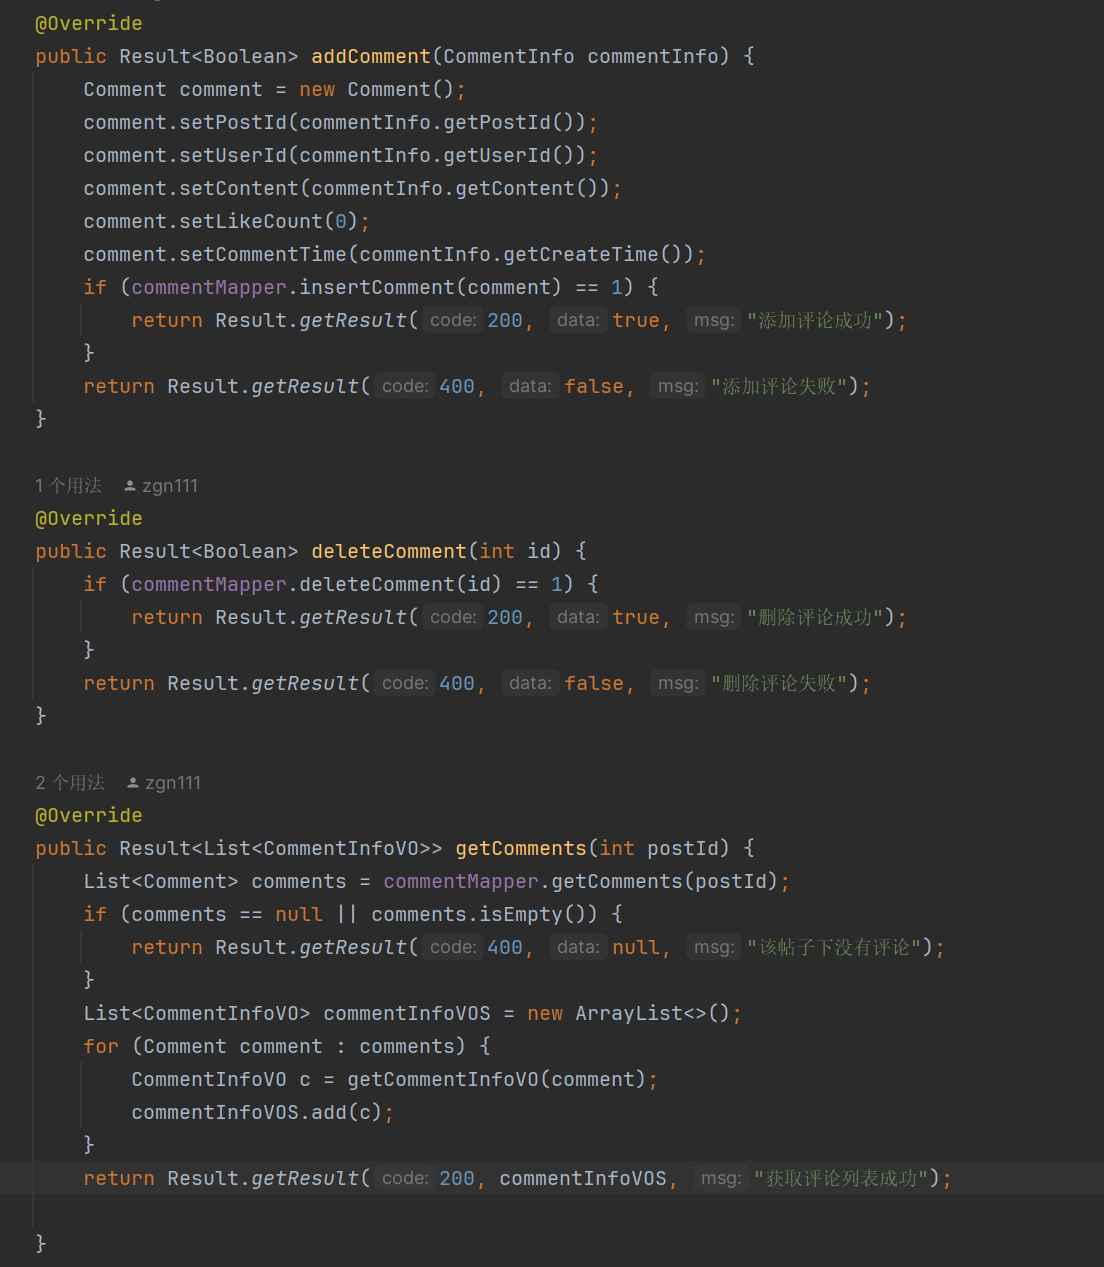
\includegraphics[scale=0.3]{系统实现/评论功能实现.png}
  \caption{评论管理功能实现}
\end{figure}

\subsubsection{模块管理功能实现}

\begin{figure}[H]
  \centering
  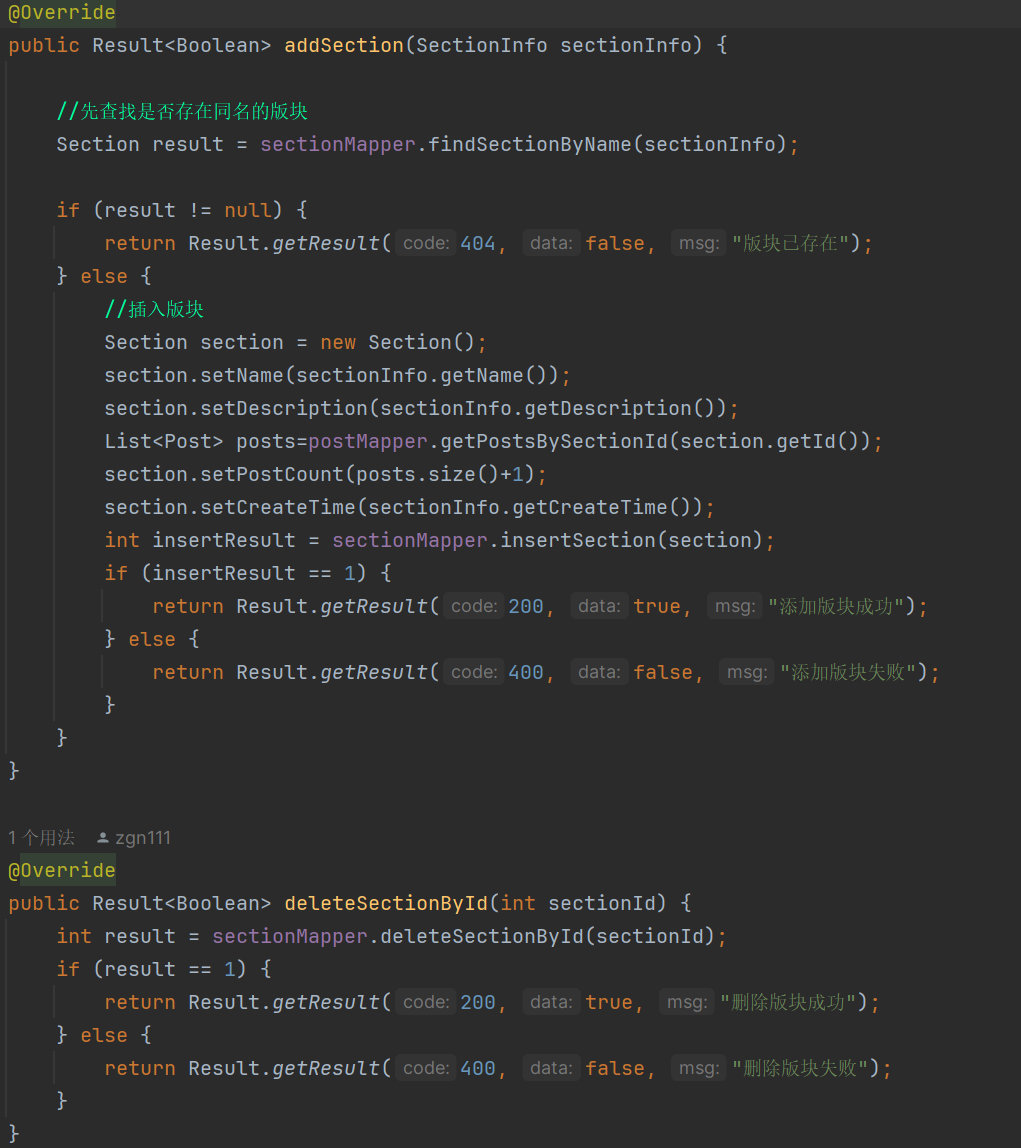
\includegraphics[scale=0.3]{系统实现/模块功能实现.png}
  \caption{模块管理功能实现}
\end{figure}


\subsection{系统测试}

\subsubsection{用户账户管理测试}

\begin{figure}[H]
  \centering
  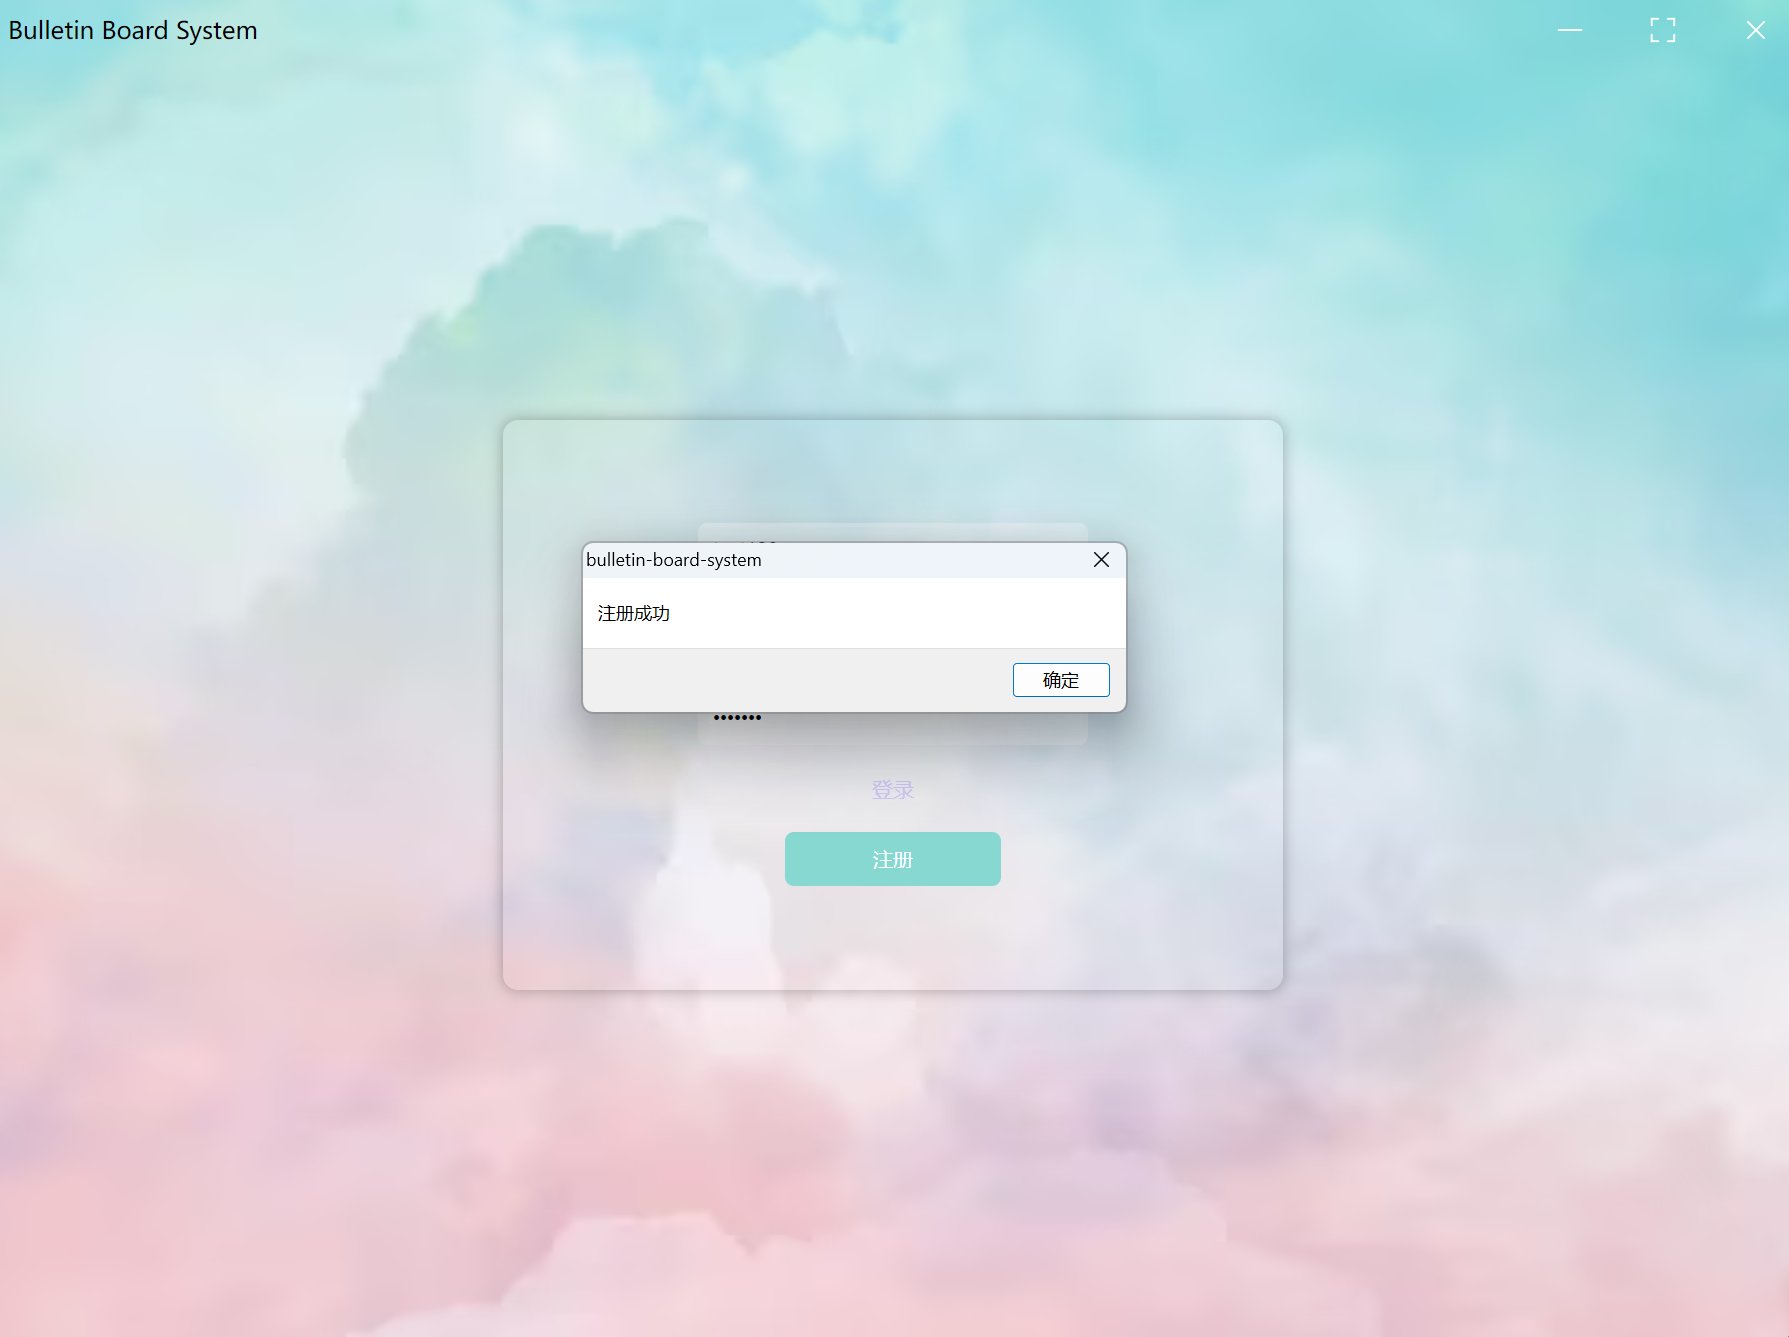
\includegraphics[scale=0.3]{测试/注册.png}
  \caption{用户注册测试}
\end{figure}

测试用例:\\
账号:test123\\
密码:test123\\

输入注册账号密码,点击注册按钮,注册成功,跳转到登录页面,可以看到后端数据库中新增了一条用户数据。

\begin{figure}[H]
  \centering
  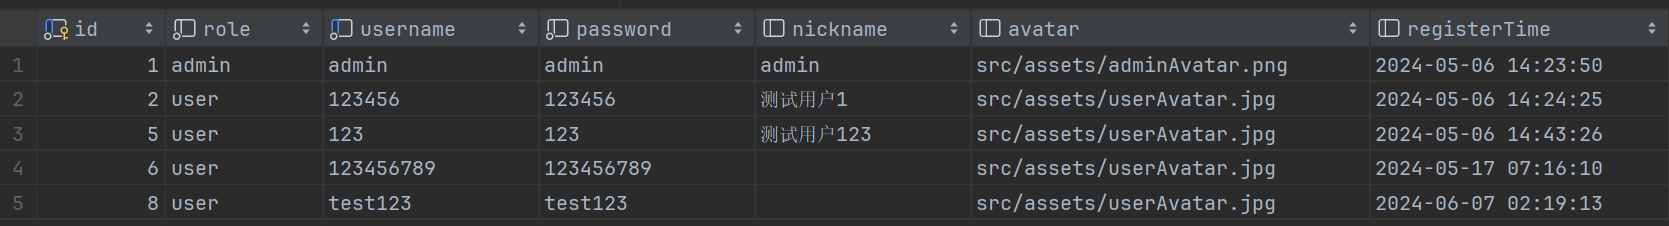
\includegraphics[scale=0.3]{测试/用户表更新.png}
  \caption{用户表更新}
\end{figure}

\begin{figure}[H]
  \centering
  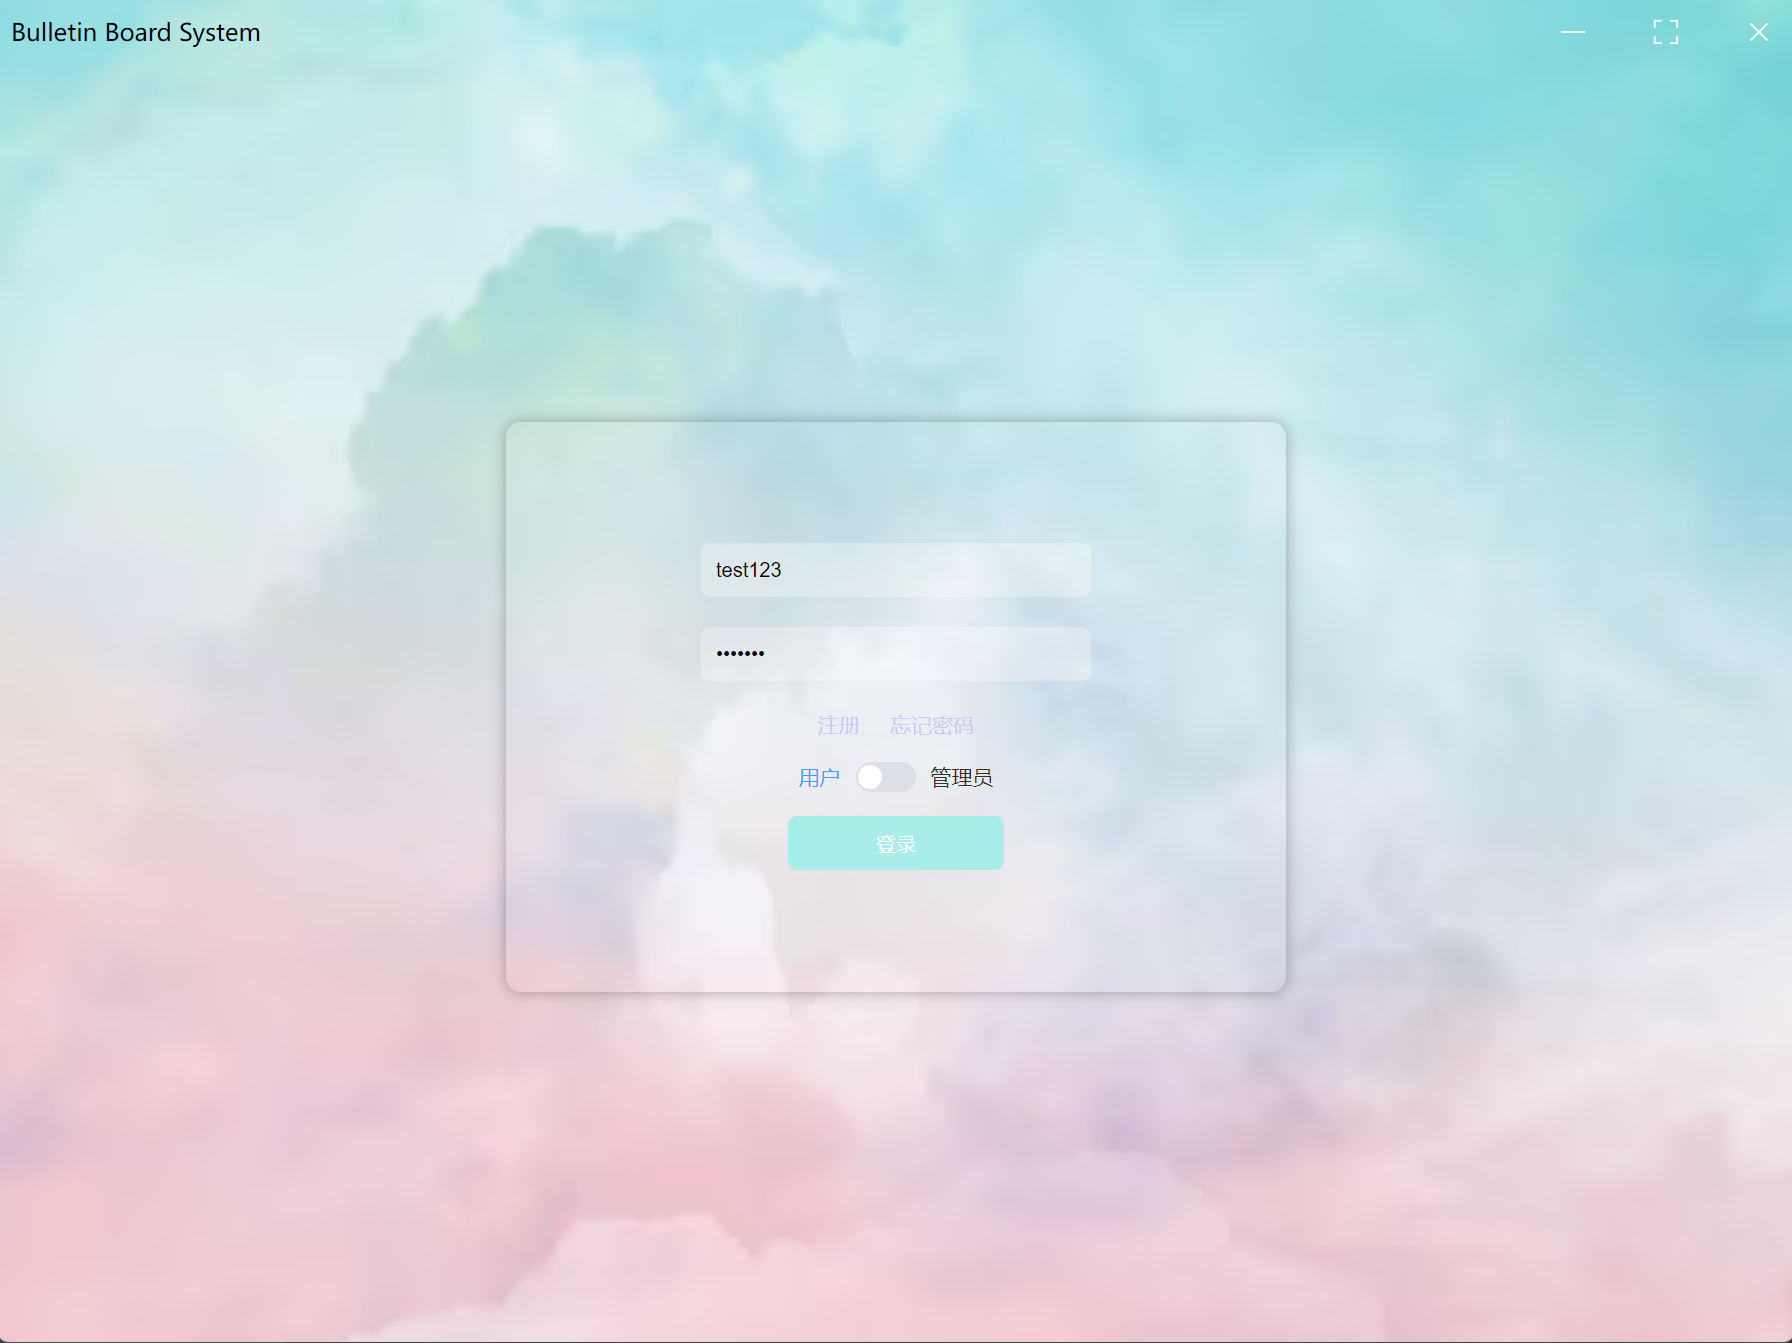
\includegraphics[scale=0.3]{测试/登录.png}
  \caption{用户登录测试}
\end{figure}

\begin{figure}[H]
  \centering
  \includegraphics[scale=0.3]{测试/管理员.png}
  \caption{管理员页面测试}
\end{figure}

管理员对于所有帖子、评论和模块都有管理权限,可以查看、删除帖子、评论和模块。

\subsubsection{帖子管理测试}

\begin{figure}[H]
  \centering
  \includegraphics[scale=0.3]{测试/发帖子.png}
  \caption{发布帖子测试}
\end{figure}

测试用例:\\
标题:测试帖子\\
内容:这是我的测试\\

输入标题和内容,点击发布按钮,发布成功,跳转到帖子页面,可以看到后端数据库中新增了一条帖子数据。

\begin{figure}[H]
  \centering
  \includegraphics[scale=0.3]{测试/帖子表更新.png}
  \caption{帖子表更新}
\end{figure}



\subsubsection{评论管理测试}

\begin{figure}[H]
  \centering
  \includegraphics[scale=0.3]{测试/评论成功.png}
  \caption{评论测试}
\end{figure}

测试用例:\\
内容:测试评论\\

输入评论内容,点击评论按钮,评论成功,可以看到后端数据库中新增了一条评论数据。

\begin{figure}[H]
  \centering
  \includegraphics[scale=0.3]{测试/评论表更新.png}
  \caption{评论表更新}
\end{figure}

\subsubsection{模块管理测试}

\begin{figure}[H]
  \centering
  \includegraphics[scale=0.3]{测试/添加模块.png}
  \caption{模块管理测试}
\end{figure}

测试用例:\\
模块名:测试\\
描述:测试模块\\

输入模块名和描述,点击添加按钮,添加成功,可以看到后端数据库中新增了一条模块数据。

\begin{figure}[H]
  \centering
  \includegraphics[scale=0.3]{测试/模块表更新.png}
  \caption{模块表更新}
\end{figure}





\newpage
\section{任务分工}

\begin{table}[H]
  \centering
  \begin{tabular}{|l|l|l|}
  \hline
      姓名 & 任务 & 贡献率\\ \hline
      张桂楠 & 报告撰写、系统代码实现 & 45\% \\ \hline
      余睿 & 类模型图和协作图和期末PPT制作   & 15\% \\ \hline
      纪安东 & 用例图和精细类图      & 10\%\\ \hline
      李绍东 & 时序图& 10\% \\ \hline
      王双阳 & 活动图 & 10\% \\ \hline
      顾逸 & 数据库ER图、表 & 10\% \\ \hline
  \end{tabular}
  \caption{任务分工}
\end{table}




\newpage
\section{总结与体会}

\subsection{总结}

本次课程设计中,我们设计并实现了一个企业级BBS系统,系统包括用户账户管理、帖子管理、评论管理、模块管理等功能。我们使用了SpringBoot框架和vue框架,实现了前后端分离。
与上学期的期末项目相比,本次课程设计中,我在实现技术方面学到了很多更新的知识,我采用了Electron框架,实现了一个桌面应用程序;其次,这次的界面设计很多都没有使用前端组件库,
而是自己手写了一些组件,这样可以更好地理解前端的原理。总的来说,这次课程设计让我学到了很多新的知识,提高了我的技术水平。
同时,这次课程设计也让我更加深入地理解了软件工程的一些概念,比如需求分析、设计、实现、测试等。
总之,这次课程设计让我受益匪浅。


\end{document}